\documentclass[../main.tex]{subfiles}

\begin{document}

In \citet{lei62velocity} si osserva che la superficie solare ha scale spazio-temporali privilegiate: in particolare \'e presente un comportamento periodico nell'atmosfera a tutte le altezze rilevato tramite effetto doppler. Il periodo \'e di circa 300 secondi e la lunghezza caratteristica di qualche \si{\mega\meter}.

Il modello proposto da \citet{ulrich70five} e \citet*{stein71five} considera le propriet\'a dei modi normali non radiali di oscillazione del Sole, in particolare usando la relazione di dispersione per onde acustiche, si ha la definizione di cavit\'a risonanti all'interno del Sole: la variazione delle propriet\'a del gas delimita le regioni di propagazione a diverse profondit\'a a seconda delle caratteristiche trasversali del moto.

In questa sezione ricavo l'equazione del moto perturbato che descrive i modi normali del Sole: considero piccole perturbazioni dello stato di equilibrio e adiabatiche cio\'e molto pi\'u rapide del tempo scala per scambio di calore dovuto al flusso radiativo o alle reazioni nucleari; e descrivo qualitativamente il diverso comportamento dei modi di gravit\'a e pressione.

In questa parte uso \cite{chr02helioseismology}, \cite{dal03notes} per la descrizione dei modi normali adiabatici e le loro propriet\'a asintotiche, \cite{appourchaux2011crash} per l'analisi dei dati.


{\let\clearpage\relax\let\cleardoublepage\relax
\chapter{Modi normali della struttura solare.}
}

\begin{workout}[cito JCD-helio02, dalsnote-stellar pulsation, AB-non asymptotic inversion]
In questo capitolo seguo 
\end{workout}

\section{Perturbazione dello stato di equilibrio.}

Descrivo le oscillazioni come piccole perturbazioni dello stato di equilibrio; in particolare considero l'equazione del moto per un elemento di fluido sottoposto a uno spostamento infinitesimo dalla posizione di equilibrio al termine lineare nelle perturbazioni nel sistema di riferimento dell'elemento.
%(gli effetti non lineari, fra cui lo scambio di energia tra i modi, sono dell'ordine di $\frac{v}{c_s}$ dove v \'e l'ampiezza della velocit\'a dell'oscillazione). 
In generale pu\'o essere presente un campo di velocit\'a $\vec{v}_0$:
\begin{align}
&\vec{v}=\vec{v}_0+\vec{v}'\intxt{con $\vec{v}'$ perturbazione euleriana della velocit\'a. La variazione di una grandezza euleriana nel riferimento solidale con l'elemento di fluido si esprime tramite:}
&\TDof{t}=\PDof{t}+(\vec{v}\cdot\nabla)
\end{align}
in prima approssimazione prendo $\vec{v}_0=0$ per poi considerare come perturbazioni gli effetti dovuti a campi di velocit\'a in specie rotazione.

Lo spostamento infinitesimo $\vec{\xi}$ dalla posizione di equilibrio determina perturbazioni nella densit\'a e nella pressione: indico con $P'(\vec{r},t)$ e $\delta P$ la perturbazione euleriana e lagrangiana della pressione e con $\rho'$, $\Phi'$ e $\vec{g}'$ la perturbazione euleriana della densit\'a , e le perturbazioni euleriane del potenziale gravitazionale e dell'accelerazione di gravit\'a conseguenti, con:
\begin{align}
&\vec{g}'=-\nabla\Phi'\\
&\nabla^2\Phi'=4\pi G\rho'\label{eq:gapert}
\end{align}
%Il valore attuale della pressione \'e la sovrapposizione del valore di equilibrio e della perturbazione:
Scrivo la pressione come somma della pressione di equilibrio e della perturbazione euleriana indicata con l'apice:
\begin{align}
&P(\vec{r},t)=P_0(\vec{r})+P'(\vec{r},t)\label{eq:pressureperturbation}\intxt{quindi per la perturbazione lagrangiana risulta:}
&\Lvar{P(\vec{r})}=P(\vec{r}+\Lvar{\vec{r}})-P_0(\vec{r})=P'(\vec{r})+\Lvar{\vec{r}}\cdot\nabla P_0
\end{align}
mentre integrando l'equazione di continuit\'a rispetto al tempo ottengo la relazione:
\begin{equation}
\rho'+\div{(\rho_0\Lvar{\vec{r}})}=0\label{eq:contper}
\end{equation}

Ricavo l'equazione del moto perturbato considerando solo i termini lineari nella perturbazione:
\begin{equation}
\rho_0\TDof{t}\vec{v}=\rho_0\PtwoDy{t}{\Lvar{\vec{r}}}=-\nabla P'+\rho_0\vec{g}'+\rho'\vec{g}_0\label{eq:emper}
\end{equation}
dove ho utilizzato la condizione di equilibrio idrostatico.

\section{Oscillazioni lineari adiabatiche.}

%Per un corpo in equilibrio idrostatico ricavo il valore medio della velocit\'a del suono utilizzando il teorema del viriale
%\begin{equation}
%\begin{split}
%&-\Omega=3\int_VP\,dV=3\int_M\frac{P}{\rho}\,dm\\
%&=3\int_M\frac{c_s^2}{\Gamma_1}\,dm=3\exv{\frac{c_s^2}{\Gamma_1}}M\approx3\frac{\overline{c}_s^2}{\Gamma_1}M
%\end{split}
%\end{equation}
%Per stelle in sequenza principale ho $\Omega=-q\frac{GM^2}{R}$ con $q\approx1.5$; per il modo fondamentale di oscillazione radiale si ha:
%\begin{equation}
%\lambda_1\approx 2\rsun{},\ \omega_1\approx\frac{c_s}{\lambda_1},\ \Pi_1\approx\SI{1}{\hour}
%\end{equation}
%dove il quadrato della velocit\'a del suono \'e
%\begin{equation}
%c_s^2=\frac{\Gamma_1P_0}{\rho_0}\label{eq:soundspeed}
%\end{equation}

L'equazione di conservazione dell'energia interna \eqref{eq:primatemp}, esplicitando il bilancio di calore \eqref{eq:heatgl}, \'e

\begin{equation}
\TDy{t}{T}-\frac{\Gamma_2-1}{\Gamma_2}\frac{T}{P}\TDy{t}{P}=\frac{1}{c_P}(\epsilon-\frac{1}{\rho}\scap{\nabla}{F})
\end{equation}

Mostro schematicamente che il termine a destra \'e trascurabile su tempi del periodo delle oscillazioni solari.


Stimo il tempo caratteristico $\tau_R$ per flusso radiativo dovuto al secondo termine del membro di destra dell'equazione precedente utilizzando \eqref{eq:radiativeflux}, con $H$ lunghezza caratteristica per la variazione di T:

\begin{minipage}[c]{0.5\textwidth}
\begin{align*}
&\frac{1}{\rho c_P}\nabla\cdot(\frac{4acT^3}{3\kappa\rho}\nabla T)\approx\frac{4acT^4}{3\kappa\rho^2c_PH^2}=\frac{T}{\tau_R}\\
&\tau_R=\num{e12}\frac{\kappa\rho^2H^2}{T^3}\ (\si{\cgs})
\end{align*}
\end{minipage}
\begin{minipage}[c]{0.5\textwidth}
\begin{tabular}{ll}
Sole&Zona convettiva\\
$\tau_R\approx\SI{e7}{\year}\approx\tkh{}$&$\tau_R\approx\SI{e3}{\year}$\\
\end{tabular}
\end{minipage}

%Sole: $\kappa=1$, $\rho=1$, $T=\num{e6}$, $H=\num{e10}$)
%Zona convettiva$\kappa=100$, $\rho=\num{e-5}$, $T=\num{e4}$, $H=\num{e9}$)
Il termine dovuto alle reazioni nucleari nell'interno solare \'e caratterizzato da un tempo $\tau_{\epsilon}\approx\frac{c_PT}{\epsilon}\approx\SI{e7}{\year}$, che confronta l'energia disponibile per grammo con quella generata dalle reazioni di fusione per unit\'a di tempo.

I tempi scala per scambio di calore nell'interno solare sono molto maggiori del periodo delle oscillazioni quindi l'approssimazione adiabatica \'e giustificata mentre non \'e pi\'u valida vicino alla superficie solare dove i tempi per lo scambio di calore sono pi\'u brevi.

Il moto di una elemento di fluido \'e descritto dalla relazione adiabatica
\begin{equation}
\TDy{t}{P}=\frac{\Gamma_1P}{\rho}\TDy{t}{\rho}
\end{equation}

\begin{figure}[!ht]

\begin{subfigure}[b]{0.47\textwidth}
\centering
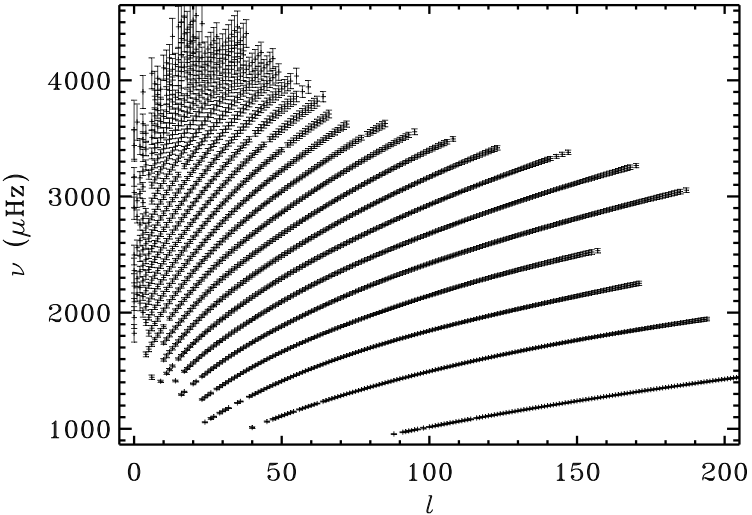
\includegraphics[keepaspectratio,width=0.95\textwidth]{midlmodes}
\caption{I picchi della densit\'a spettrale si dispongono su creste in cui \'e concentrata la potenza in accordo al modello. Determinata usando i primi 144 giorni di osservazione di MDI con $l\leq300$. Da \cite{chr02helioseismology}.}\label{fig:midlmodes}
\end{subfigure}
~
\begin{subfigure}[b]{0.5\textwidth}
\centering
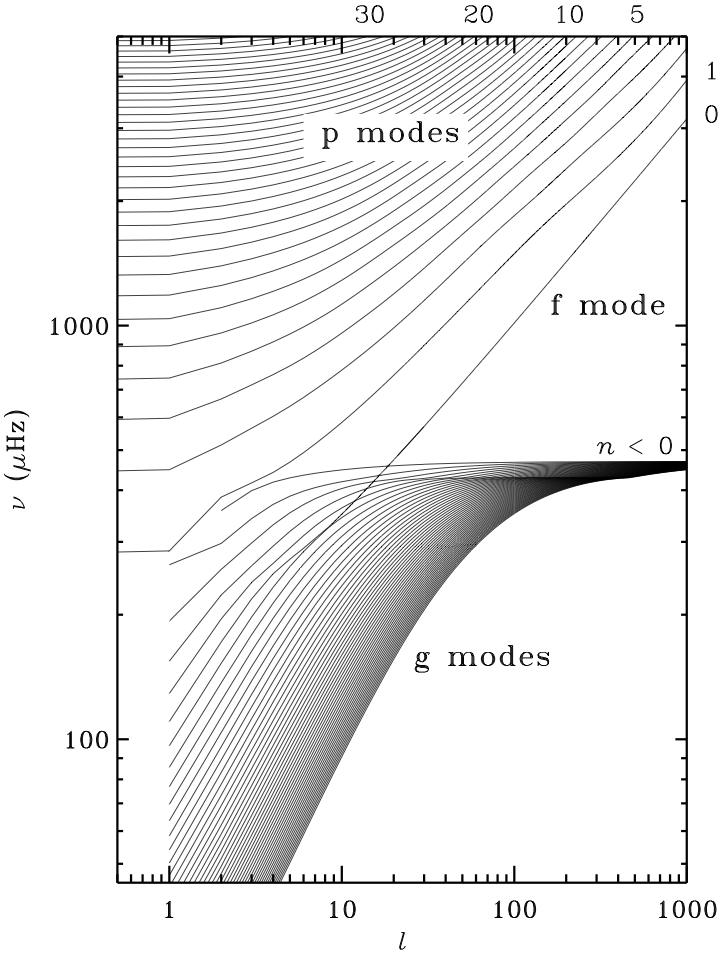
\includegraphics[keepaspectratio,width=0.95\textwidth]{nrmodesLAWE}
\caption{Modi adiabatici calcolati sulla base di un modello solare. Da \cite{chr02helioseismology}.}\label{fig:nrmodesLAWE}
\end{subfigure}

\end{figure}

La condizione di perturbazione adiabatica linearizzata \'e:
\begin{align}
&\PDy{t}{\Lvar{P}}-\frac{\Gamma_{1,0}P_0}{\rho_0}\PDy{t}{\Lvar{\rho}}=0\intxt{che integrata rispetto a t ed in funzione della variazione euleriana diventa}
&P'+\vec{\xi}\cdot\nabla P_0=\frac{\Gamma_{1,0}P_0}{\rho_0}(\rho'+\vec{\xi}\cdot\nabla\rho_0)\label{eq:adper}
\end{align}
Cerco una soluzione della forma di un'onda stazionaria: esprimo la dipendenza temporale tramite $\exp{i\omega t}$ e angolare tramite le funzioni armoniche sferiche $Y_{lm}(\theta,\phi)$ con:
\begin{align}
&Y_{lm}(\theta,\phi)=(-)^mc_{lm}P_l^m(\cos{\theta})\exp{im\phi}\\
&L^2Y_l^m=-\frac{1}{\sin{\theta}}\PDof{\theta}(\sin{\theta}\PDy{\theta}{Y_l^m})+\frac{1}{\sin^2{\theta}}\PtwoDy{\phi}{Y_l^m}=-r^2\nabla_h^2Y_l^m=l(l+1)Y_l^m\label{eq:SHperturb}
\end{align}
e scrivo la variazione euleriana di densit\'a, pressione e potenziale gravitazionale nella forma
\begin{equation}
(\rho',P',\Phi')=\exp{i\omega t}[\rho'(r),P'(r),\Phi'(r)]Y_l^m
\end{equation}


\begin{workout}[Spostamento perturbato senza L a dividere]
\begin{equation}
\vec{\xi}=\exp{i\omega t}(\xi_r(r),\frac{\xi_h(r)}{L}\PDof{\theta},\frac{\xi_h(r)}{L\sin{\theta}}\PDof{\phi})Y_l^m(\theta,\phi)
\end{equation}
\end{workout}

%inoltre, introducendo la frequenza di \bv{} (vedi \eqref{eq:bvfs}), $a=\Phi'+\frac{P}{\rho_0}$, $b=\div{\vec{\xi}}$, riscrivo l'equazione del moto \eqref{eq:emper} nella forma (vedi \citet*{ledoux1958variable})
Dall'equazione del moto \eqref{eq:emper}, poich\'e le deviazioni dalla simmetria sferica sono in prima approssimazione trascurabili, \'e evidente che:
\begin{equation}
%&\omega^2\vec{\xi}=\nabla a+\frac{N^2c^2}{g}b\frac{\vec{r}}{r}\\
\hat{r}\cdot(\rot{\vec{\xi}})=0\ \Rightarrow\ \PDof{\theta}(\sin{\theta}\xi_{\phi})-\PDy{\phi}{\xi_{\theta}}=0
\end{equation}
ed \'e quindi possibile ricavare la componente tangenziale della perturbazione da una funzione scalare. Scrivo:
\begin{equation}
\vec{\xi}=\exp{i\omega t}(\xi_r(r),\frac{\xi_h(r)}{L}\PDof{\theta},\frac{\xi_h(r)}{L\sin{\theta}}\PDof{\phi})Y_l^m(\theta,\phi)
\end{equation}
dove ho introdotto la notazione $L=\sqrt{l(l+1)}$.

Ricavo la componente $\xi_h(r)$ applicando la parte tangenziale della divergenza all'equazione del moto:
\begin{equation}
\xi_h(r)=\frac{L}{r\omega^2}(\frac{P'(r)}{\rho_0}+\Phi'(r))
\end{equation}
infine $\xi_r(r)$, $P'(r)$ e $\Phi'(r)$ sono determinati da
\begin{subequations}\label{eigenomega}
\begin{align}
&\frac{1}{r^2}\TDof{r}(r^2\xi_r)-\frac{\xi_rg_0}{c_s^2}+\frac{1}{\rho_0}(\frac{1}{c_s^2}-\frac{l(l+1)}{r^2\omega^2})P'-\frac{l(l+1)}{r^2\omega^2}\Phi'=0\\
&\frac{1}{\rho_0}(\TDof{r}+\frac{g_0}{c_s^2})P'-(\omega^2-N^2)\xi_r+\TDy{r}{\Phi'}=0\\
&\frac{1}{r^2}\TDof{r}(r^2\TDy{r}{\Phi'})-\frac{l(l+1)}{r^2}\Phi'-\frac{4\pi G\rho_0}{g_0}N^2\xi_r-\frac{4\pi G}{c_s^2}P'=0
\end{align}
\end{subequations}
%con $g=-\frac{1}{\rho_0}\TDy{r}{P_0}$.

Il sistema di equazione \eqref{eigenomega} ha soluzione con le opportune condizioni al contorno per un insieme discreto di valori delle frequenze, $\omega_{nlm}$. L'ordine angolare m non compare nelle equazioni quindi gli autovalori $\omega_{nlm}$ sono $2l+1$ degeneri: la degenerazione \'e rimossa nel caso si tenga conto della rotazione ($\frac{\Omega}{\omega}\approx\num{e-4}$).
%o di effetti gravitazionali di altri corpi.

\begin{workout}[Riferimenti rotazione: stix]

\end{workout}

Condizioni al contorno: sono necessarie 4 condizioni.
\begin{itemize}
\item Due condizioni per $r=0$ selezionano le soluzioni regolari:
\begin{equation}
P'=0,\ \Phi'=0
\end{equation}
Vicino a zero risulta un andamento asintotico
\begin{equation}
(l\neq0):\ \xi_r\propto r\expy{l-1};\ (l=0):\ \xi_r\propto r;P',\ \Phi'\propto r^l
\end{equation}

\item Alla superficie solare richiediamo la continuit\'a di $\Phi$ e $\nabla\Phi'$ e che non si abbia propagazione verso l'esterno.
All'esterno della stella ho $\rho'=0$ quindi scelgo la soluzione nulla a infinito dell'equazione di Poisson $\Phi'=Ar\expy{-l-1}$:
\begin{equation}
\TDy{r}{\Phi'}+\frac{l+1}{r}\Phi'=0,\ r=\rsun{}    
\end{equation}
La condizione di non propagazione oltre la fotosfera dipende dalla descrizione dell'atmosfera solare. Nella versione pi\'u semplice impongo che la variazione di pressione sia zero alla superficie perturbata della stella
\begin{align}
&\Lvar{P}=P'+\xi_r\TDy{r}{P}=0
\end{align}
\end{itemize}

\begin{workout}[L'ampiezza dei modi \'e normalizzata a all'ampiezza osservata in superficie.]

L'ampiezza dei modi \'e normalizzata a all'ampiezza osservata in superficie. o a 1 ??

L'energia totale di un modo \'e
\begin{align}
&E_{(n,l)}=\int_0^M\,dm\exv{\dvec{\xi}^2_{nl}}
%E_{\omega_0}=\int_0^M\exv{v_{osc}^2}
\intxt{e avendo normalizzato i modi in maniera opportuna si ha}
&E_{nl}=\msun{}??I_{nl}V_{nl}^2=\frac{1}{2}I_{nl}\omega_{nl}^2A_{nl}^2
\end{align}
dove $V_{nl}^2$ e $A_{nl}^2$ sono il valore quadratico medio della velocit\'a e dell'ampiezza dell'oscillazione in superficie.

\end{workout}

\begin{errata}[Normalizzazione autofunzioni a 1]

Normalizzando le autofunzioni in maniera che il modulo del vettore spostamento quadratico medio in superficie sia $\sqrt{\delta r|_{rms}^2+\delta h_{rms}^2}=1$, dove
\begin{align}
&\delta r|_{rms}^2=\exv{\vec{\xi}\cdot\hat{r}}=\frac{1}{2}|\tilde{\xi}_r|^2=\frac{1}{\Pi}\int_0^{\pi}\,dt\frac{1}{4\pi}\oint\Re{\tilde{\xi}_rY_{l,m}(\theta,\phi)\exp{-i\omega t}}^2\,d\omega\\
&\delta h_{rms}^2=\exv{|\vec{\xi}_h|^2}=\frac{1}{2}l(l+1)|\tilde{\xi}_h(r)|^2%=\frac{\delta h|_{rms}}{\delta r|_{rms}}=\frac{\sqrt{l(l+1)}}{\sigma}
\end{align}
ho la relazione tra energia cinetica del modo $E_{nl}$ e velocit\'a quadratica media superficiale $V_{nl}^2$:
\begin{equation}
E_{(n,l)}=\frac{1}{2}\int_0^M\,dm\exv{\dvec{\xi}^2_{nl}}=\frac{1}{2}I_{nl}V_{nl}^2
\end{equation}

\end{errata}

L'energia cinetica di un modo \'e
\begin{equation}
E_k^{nl}=\frac{1}{2}\int_V|\vec{v}|^2\rho_0\,dV=\frac{\omega_{nl}^2}{2}\int_V|\vec{\xi}_{nl}|^2\rho_0\,dV
\end{equation}
e la media su un periodo
\begin{equation}
\bar{E_k^{nl}}=\frac{1}{\Pi}\int_0^{\Pi}E_k^{nl}=\frac{1}{2}M_{nl}V_{nl}^2
\end{equation}
dove $V_{nl}^2$ indica la velocit\'a quadratica media superficiale e ho definito l'inerzia normalizzata e la massa di un modo come:
\begin{align}
&I_{nl}=\frac{1}{\msun{}A_{nl}^2}\int_V\,d^3x\rho_0\vec{\xi}\vec{\xi}^*\label{eq:normalizedinertia}\\
%&\exv{\vec{\xi}(R)\vec{\xi}^*(R)}
&M_{nl}=I_{nl}\msun{}\intxt{inoltre ho introdotto lo spostamento quadratico medio superficiale}
&A_{nl}^2=\delta r|_{rms}^2+\delta h_{rms}^2\intxt{con}
&\delta r|_{rms}^2=\frac{1}{\Pi}\int_0^{\pi}\,dt\frac{1}{4\pi}\oint\Re{[\xi_rY_{l,m}(\theta,\phi)\exp{-i\omega t}]}^2\,d\Omega=\frac{1}{2}|\xi_r|^2\\
&\delta h_{rms}^2=\frac{1}{2}l(l+1)|\xi_h(r)|^2%=\frac{\delta h|_{rms}}{\delta r|_{rms}}=\frac{\sqrt{l(l+1)}}{\sigma}
\end{align}


Le oscillazioni solari sono in prevalenza dovute ad onde acustiche, in cui la forza di richiamo \'e prodotta dal gradiente di pressione, modi p, e onde in cui la forza di richiamo \'e la forza di gravit\'a, i modi g: i modi osservabili pi\'u facilmente hanno periodo attorno a \SI{5}{\minute} ci\'o \'e dovuto all'aumento del rumore solare a basse frequenze e ai processi di eccitazione dei modi che trasferiscono la massima energia ai modi di tale periodo.

\begin{figure}[!ht]
\centering
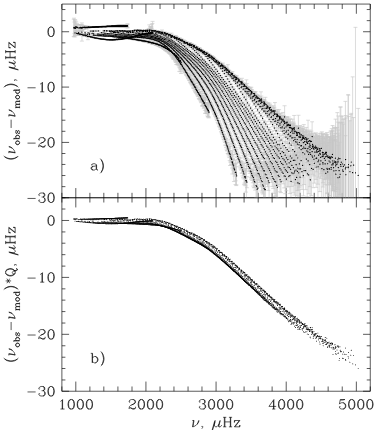
\includegraphics[keepaspectratio,width=0.9\textwidth]{domega}
\caption{In alto: differenze tra frequenze dei modi teoriche e osservate. In basso: differenze moltiplicata per $Q_{nl}$: viene rimossa la dipendenza da l dovuta alla maggiore ampiezza delle autofunzioni nelle regioni superficiali in cui l'approssimazione adiabatica non \'e corretta. Da \cite{rhodesmeasurements}.}\label{fig:nFreqdiff}
\end{figure}

Nella figura (\subref{fig:nrmodesLAWE}) sono mostrate le frequenze dei modi soluzioni del sistema \eqref{eigenomega} calcolati usando le grandezze di equilibrio di un modello solare, in (\subref{fig:midlmodes}) le frequenze misurate e in \ref{fig:nFreqdiff} le differenze tra frequenze predette e osservate.

Gli effetti dovuti alla non corretta descrizione fisica dei modi vicino alla superficie sono maggiori per i modi di l elevato perch\'e confinati in gusci meno profondi al crescere di l. 

\begin{workout}[Effetti dissipativi/propagazione di fase]

\begin{figure}[!ht]
\centering
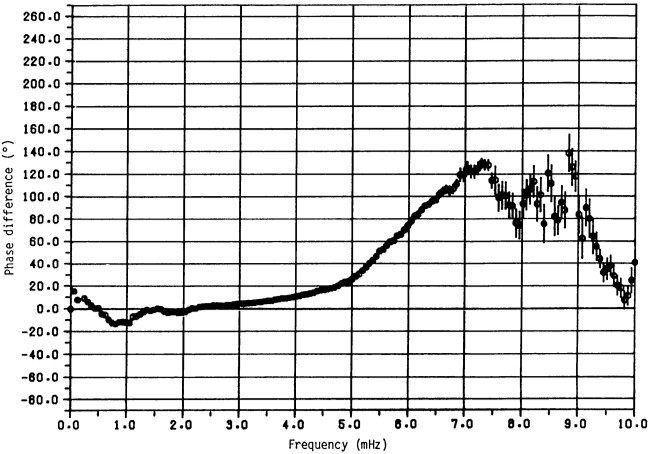
\includegraphics[keepaspectratio,width=0.9\textwidth]{phasepropagation}
\caption{Differenza di fase per il segnale Doppler delle righe $(5930)$ Fe I, pi\'u profonda, e $(5896)$ Na I, pi\'u alta nell'atmosfera. Da \cite{staiger1987observations}.}\label{fig:phasedifference}
\end{figure}

($r>0.95\rsun{}$)

\end{workout}

Introduco il rapporto d'inerzia:
\begin{align}
%&\frac{V_{nl}}{V_0(\nu_{nl})}=(Q_{nl})\expy{-\midfrac{1}{2}}\intxt{dove ho introdotto l'inerzia e il rapporto d'inerzia $Q_{nl}$}
&Q_{nl}=\frac{I_{nl}}{I^0_{nl}}\label{eq:surfaceeffects}
\end{align}
dove $I^0_{nl}$ \'e l'inerzia per un modo di frequenza $\omega_{nl}$ estrapolata a $l=0$: $Q_{nl}=1$ per $l=0$ e diminuisce al crescere di $l$. L'ampiezza superficiale relativa al modo radiale difrequenza $\nu_{nl}$
\begin{equation}
\frac{A_{nl}(\nu_{nl})}{A_{nl}^0(\nu_{nl})}\propto(Q_{nl})\expy{-\midfrac{1}{2}}
\end{equation}
cresce con l.

\begin{workout}[$\bar{E}_l(\omega)$ is obtained by interpolating in $\omega$ $E_{nl}$ at fixed l]

$\bar{E}_0(\omega_{nl})$

\end{workout}

\begin{workout}[Mode energy normalized by squared surface amplitude]

\end{workout}

Il comportamento all'aumentare della frequenza mostrato in figura (\ref{fig:nFreqdiff}) \'e dovuto al fatto che per frequenze maggiori la regione in cui si ha riflessione interna \'e pi\'u in alto dove l'approssimazione adiabatica \'e meno valida.%; la figura \subref{fig:phasedifference} mostra la propagazione di fase ad alte frequenze dovuta ad effetti dissipativi.

%in assenza di effetti dissipativi la velocit\'a di fase \'e nulla e la velocit\'a di gruppo infinita, velocit\'a e pressione sono sfasati di $\frac{\pi}{2}$..

\section{Principio variazionale}    %Vedi pg 110 dalsnote.

Riscrivo l'equazione del moto linearizzata \eqref{eq:emper}, definendo l'operatore lineare $L$ nella forma
\begin{equation}
-\omega^2\vec{\xi}=\frac{1}{\rho_0}\nabla p'-\vec{g}'-\frac{\rho'}{\rho_0}\vec{g}_0=L(\vec{\xi})\label{eq:eigenhermitian}
\end{equation}
da cui, utilizzando \eqref{eq:adper} e \eqref{eq:contper}, si ottiene
\begin{equation}\label{eq:EOMrhoc}%Unno89
-\omega^2\rho_0\xi=\nabla(c_s^2\rho_0\scap{\nabla}{\xi}+\nabla P_0\cdot\vec{\xi})-\vec{g}_0\nabla\cdot(\rho_0\vec{\xi})-G\rho_0\nabla(\int_V\frac{\nabla\cdot(\rho_0\vec{\xi})\,d^3r'}{|\vec{r}-\vec{r}'|})
\end{equation}

\citet{Cha64Variational} ha dimostrato che questo costituisce un problema agli autovalori hermitiano per condizioni ai bordi di pressione e densit\'a nulle quindi $\omega^2$ \'e reale e autofunzioni di frequenza caratteristica diversa sono ortogonali:
\begin{equation}
\int\vec{\xi}_i*\vec{\xi}_j\rho_0\,d^3x=0
\end{equation}

\'E utile scrivere la relazione tra variazioni nell'operatore lineare $L$ e differenze nelle frequenze caratteristiche:
\begin{equation}
(L+\Lvar{L})(\xi+\Lvar{\xi})=-(\omega+\Lvar{\omega})^2(\xi+\Lvar{\xi})\label{eq:EMvar}
\end{equation}
quindi considerando i termini lineari nelle variazioni e dato che le frequenze caratteristiche sono stazionarie per variazioni di $\xi$ si ha la relazione:
\begin{equation}\label{eq:variational}
\frac{\Lvar{\omega}}{\omega}=-\frac{\int_V\rho_0\vec{\xi}\Lvar{L}\vec{\xi}\,d^3x}{2\omega^2\int_V\rho_0\scap{\xi}{\xi}d^3x}
\end{equation}

\subsection{Variazioni struttura idrostatica e variazioni nell'equazione di stato e nella  composizione}

Esplicito la forma della perturbazione $\delta L$ in \eqref{eq:EOMrhoc} introducendo piccole variazioni nel profilo di $\rho$ e $c_s$:
\begin{equation}
\Lvar{L}\vec{\xi}=\nabla(\Lvar{c_s^2}\nabla\cdot\vec{\xi}+\Lvar{\vec{g}}\cdot\vec{
\xi})+\nabla(\frac{\Lvar{\rho}}{\rho_0})c^2\nabla\cdot\vec{\xi}+\frac{1}
{\rho_0}\nabla\rho_0\Lvar{c_s^2}\nabla\vec{\xi}+\Lvar{\vec{g}}\nabla\cdot\vec{\xi}-
G\nabla\int_V\frac{\nabla\cdot(\Lvar{\rho}\xi)}{|\vec{x}-
\vec{x}'|}\,d^3x'\label{eq:eqmotvar}
\end{equation}
con
\begin{equation}
\Lvar{g}(r)=\frac{4\pi G}{r^2}\int_0^r\Lvar{\rho}(s)s^2\,ds
\end{equation}

\'E quindi possibile esprimere le differenze nelle frequenze dei modi nella forma
\begin{equation}\label{eq:hydroefdiff}
\frac{\delta\omega_{nl}}{\omega_{nl}}=\int_0^R[K^{nl}_{c^2,\rho}(r)\frac{\delta_rc^2}{c^2}(r)+K^{nl}_{\rho,c^2}(r)\frac{\delta_r\rho}{\rho}(r)]\,dr+M_{nl}\expy{-1}F_{Surf}
\end{equation}

\begin{workout}[Termine superficiale e rapporto d'inerzia - AB94 NON asymptotic inversion]
\[Q_{nl}\ I_{nl}\ M_{nl}\]
\end{workout}

I kernel $K_Q^j$ dipendono dalle autofunzioni dei modi calcolati tramite il modello solare, il termine $M_{nl}\expy{-1}F_{Surf}(\omega_{nl})$ tiene conto degli effetti superficiali.

\begin{errata}[Inutile espicitare i kernel]
La forma esplicita dei kernel si ottiene sostituendo \eqref{eq:eqmotvar} in \eqref{eq:variational}:
\begin{equation}
F_{Surf}(\omega)-\frac{1}{2\omega^2}(I_1+I_2+I_3+I_4)=I_{nl}\frac{\Lvar{\omega}}{\omega}
\end{equation}
con
\begin{align}
&I_1=-\int_0^R\rho(\scap{\nabla}{\xi})^2\Lvar{c^2}r^2\,dr\\
&I_2=\int_0^R\xi_r[\rho\scap{\nabla}{\xi}+\nabla\cdot(\rho\vec{\xi})]\Lvar{g}r^2\,dr\\
&I_3=\int_0^R\rho c^2\xi_r\scap{\nabla}{\xi}\PDof{r}(\frac{\Lvar{\rho}}{\rho})r^2\,dr\\
\begin{split}
&I_4=\frac{4\pi G}{2l+1}\int_0^R\divof{}(\rho\vec{\xi})r^2\,dr[\frac{1}{r\expy{l+1}}\int_0^rs\expy{l+2}(\rho\divec{\xi}-\rho\TDy{s}{\xi_r}-\frac{l+2}{s}\rho\xi_r)\frac{\Lvar{\rho}}{\rho}\,ds\\
&+r^l\int_r^R\frac{1}{s\expy{l-1}}(\rho\divec{\xi}-\rho\TDy{s}{\xi_r}-\frac{1-l}{s}\rho\xi_r)\frac{\Lvar{\rho}}{\rho}\,ds]
\end{split}
\end{align}
\end{errata}

\begin{workout}[correzioni non infinitesime]
Nel caso l'entit\'a delle correzioni a $\rho$ e $c^2$ non giustifichi l'approssimazione lineare si ha un miglior accordo definendo la differenza tramite $\frac{\Lvar{f}}{f}=\frac{f-f_0}{\sqrt{ff_0}}$.
\end{workout}

Le variazioni della pressione si ottengono dall'equazione di equilibrio idrostatico \eqref{eq:fidroequilibrio}
\begin{equation}
\Lvar{P}=\int_r^R(g\Lvar{\rho}+\rho\Lvar{g})\,dr\label{eq:pressurecorrho}
\end{equation}

%\subsection{Inversione equazione di stato e composizione.}

Per investigare la composizione \'e necessario usare l'equazione di stato per esplicitare $\Gamma_1(P,\rho,X_i)$. Riscrivo \eqref{eq:hydroefdiff} nella forma:
\begin{equation}
\frac{\delta\omega_{nl}}{\omega_{nl}}=\int_0^RK^{nl}_{u,\Gamma_1}(r)\frac{\delta_ru}{u}(r)\,dr+\int K^{nl}_{\Gamma_1,u}(r)\delta_r\frac{\delta_r\Gamma_1}{\Gamma_1}\,dr+M_{nl}\expy{-1}F_{Surf}(\omega_{nl})\label{eq:invdGammadrho}
\end{equation}
per la coppia di variabili $(u=\midfrac{P}{\rho},\Gamma_1)$ e formula analoga esiste per le variabili $(\Gamma_1,\rho)$.
\'E possibile esplicitare, tramite l'equazione di stato, la dipendenza di $\Gamma_1$ dalla composizione chimica; in particolare si ha:
\begin{equation}
\frac{\delta\omega_{nl}}{\omega_{nl}}=\int_0^RK^{nl}_{u,Y}(r)\frac{\delta_ru}{u}(r)\,dr+\int K^{nl}_{Y,u}(r)\delta_rY\,dr+\int_0^RK^{nl}_{c^2,\rho}(r)(\frac{\delta\Gamma_1}{\Gamma_1})_{int}\,dr+I_{nl}\expy{-1}F_{Surf}(\omega_{nl})\label{eq:diffthermo}
\end{equation}
dove si tiene conto degli errori sistematici dovuti alle discrepanze nell'equazione di stato e nella metallicit\'a tramite $(\delta\Gamma_1)_{int}$, differenze nell'equazione di stato a $(P,\rho,Y)$ fissati.

La determinazione dell'abbondanza di elio nella regione convettiva \'e dovuta principalmente alla deviazione da $\Gamma_1=\frac{5}{3}$ nella regione di seconda ionizzazione dell'elio.

\begin{workout}[Esplicito dipendenza di $\Gamma_1(P,\rho,X_i)$]

\begin{equation}
\frac{\delta\Gamma_1}{\Gamma_1}=(\PDy{Y}{\ln{\Gamma_1}})_{(P,\rho)}\delta Y+(\PDy{P}{\ln{\Gamma_1}})_{(\rho,Y)}\frac{\delta P}{P}+(\PDy{\rho}{\ln{\Gamma_1}})_{(P,Y)}\frac{\delta\rho}{\rho}+(\frac{\delta\Gamma_1}{\Gamma_1})_{Int}
\end{equation}

\end{workout}

\begin{workout}[citare B-jcd 97]

\end{workout}

\begin{workout}[coerenza: in questa parte solo differenze frequenze ($Y_{CZ}$]
La determinazione dell'abbondanza di elio nella regione convettiva \'e dovuta principalmente alla deviazione da $\Gamma_1=\frac{5}{3}$ nella regione di seconda ionizzazione dell'elio.
risulta $Y_{CZ}=\num{0.2485+-0.0034}$.
\end{workout}

%Esprimendo $\delta_rc^2$ in termini di $\delta_ru=\delta_r(\frac{P}{\rho})$, $\delta_rY$ e $\delta_r\Gamma_1$, riscriviamo \eqref{eq:invstructure}, dove abbiamo utilizzato l'equazione di stato per descrivere la dipendenza di $\Gamma_1$ dall'abbondanza di $\cel{He}{4}{}{}$:
% Dals Art pg 31-32
%Le differenze in $U$ e $\rho$  fra modelli solari sismologici e modelli solari standard sono al massimo pochi per cento.

\begin{workout}[Spostare ordine: qui propriet\'a asintotiche]

\end{workout}


{\makeatletter\let\ps@chapter\ps@plain\makeatother
\let\clearpage\relax\let\cleardoublepage\relax%%% Chapter  Caratteristiche asintotiche delle oscillazioni adiabatiche.
\chapter{Caratteristiche asintotiche delle oscillazioni adiabatiche.}\label{chap:asyntoticbehavour}
}

\begin{workout}[Classificazione modi: approx cowling (parametrizzation)]

\end{workout}

I modi gravo-acustici descritti in \eqref{eigenomega} si riducono ai modi p ed f per alte frequenze e ai modi g per basse frequenze. Approssimando il comportamento della perturbazione localmente con un'onda piana e trascurando la perturbazione al potenziale gravitazionale $\Phi'$ si ottendono soluzioni asintotiche per i modi normali e relazioni di dispersione approssimate.

\section{Soluzione asintotica dei modi.}

L'approssimazione di Cowling (\cite{cow41oscillations}) consiste nel trascurare la perturbazione al potenziale gravitazionale
\begin{equation}
\Phi'(r)=-\frac{4\pi G}{2l+1}\left[\frac{1}{r^{l+1}}\int_0^r\rho'(r)r'^{l+2}\,dr'+r^l\int_r^R\frac{\rho'(r')}{r'^{l-1}}\,dr'\right]\label{eq:perturbedgravitational}
\end{equation}

da cui si vede che $|\Phi'|$ \'e trascurabile rispetto a $\rho'$ sia nel caso in cui $l\gg1$, per l'esponente crescente con l al denominatore dei due addendi in \eqref{eq:perturbedgravitational}, sia nel caso $|n|\gg1$, per il comportamento rapidamente oscillante di $\rho'$.

Il sistema \eqref{eigenomega} si riduce a:
\begin{subequations}\label{cowosc:main}
\begin{align}
&\frac{1}{r^2}\TDof{r}(r^2\xi_r)-\frac{\xi_rg_0}{c_s^2}+\frac{1}{\rho_0}(\frac{1}{c_s^2}-\frac{l(l+1)}{r^2\omega^2})P'=0\label{cowosc:a}\\
&\frac{1}{\rho_0}(\TDof{r}+\frac{g_0}{c_s^2})P'-(\omega^2-N^2)\xi_r=0\label{cowosc:b}
\end{align}
\end{subequations}
%Cowling approx dalsnotes:
%\begin{subequations}
%\begin{align}
%&\TDy{r}{\xi_r}=-(\frac{2}{r}-\frac{1}{\Gamma_1}\invers{H_p})\xi_r+\frac{1}{\rho_0c^2}(\frac{S_l^2}{\omega^2}-1)P'\\
%&\TDy{r}{P'}=\rho_0(\omega^2-N^2)\xi_r+\frac{1}{\Gamma_1}\invers{H_p}P'\\
%\end{align}
%\end{subequations}

Considero i limiti asintotici di alte e basse frequenze: ottengo un problema del tipo di Sturm-Liuville.
%https://en.wikipedia.org/wiki/Sturm%E2%80%93Liouville_theory
\begin{itemize}
\item Per $\omega\to\infty$: lo spettro \'e discreto, le oscillazioni sono prodotte da onde acustiche in cui la forza dominante \'e fornita dalla pressione, i modi p, ordinati in base al numero di zeri di $\xi_r$ fra il centro e la superficie.

\item Per $\omega\to0$ lo spettro \'e discreto, il moto \'e determinato dalla forza di gravit\'a: si hanno i modi g.

\end{itemize}
%Lo spettro solare \'e la combinazione dei modi parziali precedenti; 
I modi f separano i modi g e p: non hanno nodi in direzione radiale.

\section{Relazione di dispersione per i modi gravo-acustici.}

Approssimo il comportamento spaziale delle oscillazioni localmente con un'onda piana $\vec{\xi}\propto\exp{i\scap{k}{x}}$ con $\vec{k}=k_r\hat{r}+\vec{k}_h$.

\'E utile fare l'ulteriore approssimazione, valida per grandi n, di trascurare la variabile perturbata rispetto alla sua derivata radiale, e cos\'i si ottiene
\begin{equation}\label{eq:secondorder}
\TtwoDy{r}{\xi_r}=\frac{\omega^2}{c_s^2}(1-\frac{N^2}{\omega^2})(\frac{S_l^2}{\omega^2}-1)\xi_r=-K(r)\xi_r
\end{equation}
per $K(r)>0$ quest'equazione descrive un comportamento oscillante. Si ha la relazione di dispersione:
\begin{equation}
k_r^2=\frac{\omega^2}{c_s^2}(1-\frac{N^2}{\omega^2})(1-\frac{S_l^2}{\omega^2})\label{eq:approximatedispersion}
\end{equation}

Le approssimazioni fatte non sono pi\'u valide vicino alla superficie dove il termine in $\invers{H_P}$ non \'e trascurabile per $H_P$ piccolo e vicino al centro solare dove il termine in $\frac{2}{r}$ non \'e trascurabile.

Considero \eqref{cowosc:main}  per lunghezza d'onda delle perturbazioni molto minore della scala caratteristica di variazione di $N, c$.
%stix local treatment pg 165

\begin{workout}[Unire relazione dispersione e cavit\'a risonanti]
e levare tentativo deduzione $\omega_c$
\end{workout}

\begin{workout}[Costanza del flusso: densit\'a di energia per velocit\'a di gruppo]

\begin{align}
&\xi_r\propto\rho_0\expy{-1/2}\exp{ik_rr},\ P_1\propto\rho_0\expy{1/2}\exp{ik_rr}
\end{align}

Ulrich70/landau fluid $\S49$/dalsnotes Pg 127 chapt 7
Uso che $\vec{\xi}$ e $\delta P$ sono sfasati di $90$

Work\[-\int_0^{2\pi/\omega}v_zP'\,dt\]
Therma flux\[-\int_0^{2\pi/\omega}\rho v_zE\,dt\]
Thermal energy density\[-\int_0^{2\pi/\omega}[\rho E-(\rho E)_0]\,dt\]
KE density\[-\int_0^{2\pi/\omega}\frac{1}{2}\rho v^2\,dt\]
\[-\int_{z_1}^{z_2}[\text{Energy density}]\,dz=F(z_1)-F(z_2)\]

\end{workout}

\begin{workout}[Equazione oscillazioni con $\omega_c$:Gough-deubner84 dalsnotes chap7]

Sostituisco
\begin{align}
&\xi_r\propto\rho_0\expy{-\frac{1}{2}}\exp{ik_rr},\ P_1\propto\rho_0\expy{\frac{1}{2}}\exp{ik_rr}\intxt{dove la dipendenza dalla densit\'a di equilibrio \'e dovuta alla conservazione dell'energia. Definisco la frequenza critica acustica:}
&\omega_c=\frac{c_s}{2\densityscale{}}\sqrt{1-2\TDy{r}{\densityscale{}}}\propto T\expy{-\frac{1}{2}}\label{eq:acusticcutoff} \intxt{quindi ottengo la relazione di dispersione:}
&k_r^2=\frac{\omega^2-\omega_c^2}{c^2}+S_l\frac{N^2-\omega^2}{c^2\omega^2}=\frac{\omega^2}{c^2}(1-\frac{\omega_{l,+}^2}{\omega^2})(1-\frac{\omega_{l,-}^2}{\omega^2})\label{eq:localdispersion}\intxt{dove ho definito le frequenze critiche per i modi gravo-acustici}
&\omega_{\pm}=\frac{1}{2}(S_l^2+\omega_c^2)\pm\sqrt{\frac{1}{2}(S_l^2+\omega_c^2)^2-N^2S_l^2}
\end{align}

\end{workout}

Per descrivere la riflessione superficiale si risolve il sistema di Cowling senza trascurare alcun termine; introduco la frequenza critica acustica 
\begin{equation}
\omega_c=\frac{c_s}{2\densityscale{}}\sqrt{1-2\TDy{r}{\densityscale{}}}\propto T\expy{-\frac{1}{2}}\label{eq:acusticcutoff}
\end{equation}
e si trova la relazione di dispersione che per frequenze acustiche prevede un punto di inversione per $\omega=\omega_c$
\begin{align}
&k_r^2=\frac{\omega^2-\omega_c^2}{c^2}+S_l\frac{N^2-\omega^2}{c^2\omega^2}=\frac{\omega^2}{c^2}(1-\frac{\omega_{l,+}^2}{\omega^2})(1-\frac{\omega_{l,-}^2}{\omega^2})\label{eq:localdispersion}\intxt{dove ho definito le frequenze critiche per i modi gravo-acustici}
&\omega_{\pm}=\frac{1}{2}(S_l^2+\omega_c^2)\pm\sqrt{\frac{1}{2}(S_l^2+\omega_c^2)^2-N^2S_l^2}
\end{align}
per cui nell'interno solare, soprattutto per grandi l, vale
\begin{equation}
\omega_{l,+}\approx S_l\ \omega_{l,-}\approx N
\end{equation}
e vicino alla superficie
\begin{equation}
\omega_{l,+}\approx \omega_c\ \omega_{l,-}\approx 0
\end{equation}

\section{Cavit\'a risonanti.} \label{sec:resonantcavity} %Definizione frequenze critiche

I modi p e g sono confinati in regioni dell'interno solare determinate dalla variazione delle caratteristiche del plasma solare.
%La variazione delle propriet\'a del gas influenzano la velocit\'a del suono, $c_s=\Gamma_1\frac{P}{\rho}$, e le frequenze critiche: esistono regioni dell'interno solare, dipendenti dalla natura delle oscillazioni, in cui \'e possibile un comportamento periodico ai cui bordi si ha riflessione interna.

\begin{minipage}{\linewidth}
\begin{tikzpicture}
\node[inner sep=0pt] (image) at (-0.5,0)
  {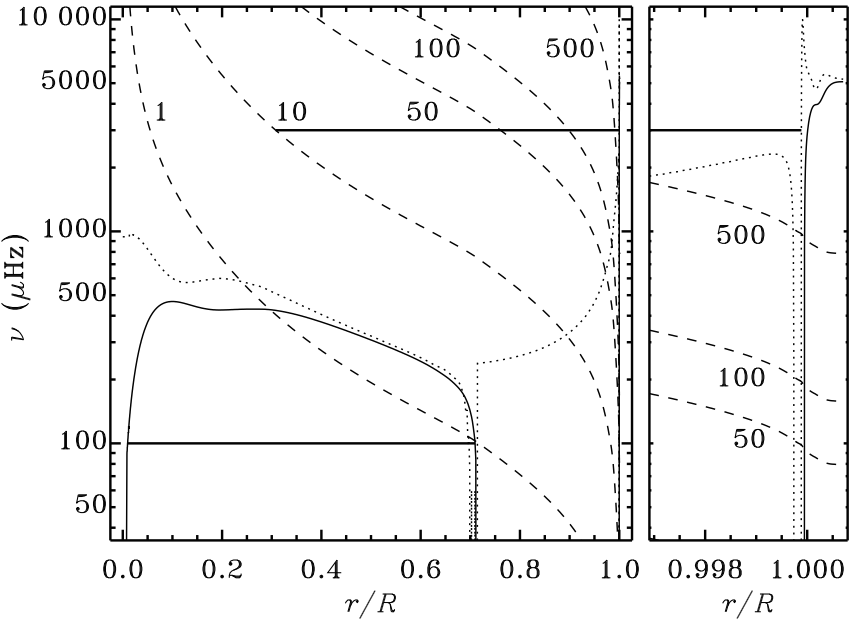
\includegraphics[keepaspectratio=true,scale=0.35]{cutoff}};
  \node (legenda) at (5.8,3) { Legenda };
  \draw [draw=black!50] (legenda.north west) rectangle +(0.35\textwidth, -4cm);
  \draw [dotted] (6,2) -- (5.5,2) node[at start, anchor=west] {$\frac{\omega_c}{2\pi}$;};
  \draw [dashed] (7.5,2) -- (7,2) node[at start, anchor=west] {$\frac{S_l}{2\pi}$;};
  \draw [] (9,2) -- (8.5,2) node[at start, anchor=west] {$\frac{N}{2\pi}$;};
  \node at (7.9,0.5) {\parbox{0.32\textwidth}{Le linee orizzontali a \SI{100}{\micro\hertz} e \SI{3000}{\micro\hertz} demarcano le regione in cui sono confinati risp. un modo g e p.}};
  \node (caption) at (7.6,-2.3) { \begin{minipage}[l]{0.3\textwidth}
\captionof{figure}{Frequenze caratteristiche calcolate tramite il modello S. Da \cite{chr02helioseismology}.\label{cutoff}}%   
    \end{minipage}};
\end{tikzpicture}
\end{minipage}

\begin{wrapfigure}[17]{r}{0.4\textwidth}
\centering
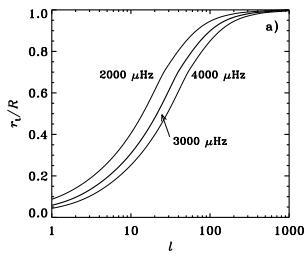
\includegraphics[keepaspectratio,angle=0,width=0.4\textwidth]{plowertp}
\caption{Andamento del raggio di inversione del moto in funzione del grado l. Da \cite{dal03notes}.}\label{fig:plowertp}
\end{wrapfigure}

Le onde acustiche sono confinate in una regione che \'e limitata superiormente dall'aumento della frequenza critica acustica
\begin{equation}
\omega_c=\frac{c_s}{2\densityscale{}}\sqrt{1-2\TDy{r}{\densityscale{}}}\propto T\expy{-\frac{1}{2}}\label{eq:acusticcutoff}
\end{equation}
 causato dalla diminuzione della temperatura che provoca la riflessione delle onde con periodo attorno ai 5-min, mentre l'aumento della velocit\'a del suono con la profondit\'a e la conseguente rifrazione dell'onda porta a propagazione del moto puramente tangenziale $k_r=0$ nel guscio sferico per cui $c_s=\frac{\omega}{k_h}\approx\omega \frac{r}{L}$ ovvero per $\omega=S_l$ frequenza di Lamb definita da
\begin{equation}
S_l^2=\frac{l(l+1)c_s^2}{r^2}\label{eq:Lambf}
\end{equation}
Definisco il raggio di inversione del moto tramite:
%Si pu\'o stimare la profondit\'a della cavit\'a acustica, utilizzando la condizione $c_s=\frac{\omega}{k_h}$ per $k_r=0$: approssimo la temperatura al punto di inversione del moto con $T\approx\Dcvar{\TDy{r}{T}}{ad}\delta$ dove $\delta$ \'e la profondit\'a della cavit\'a e, ipotizzando un gas ideale, ho $\Dcvar{\TDy{r}{T}}{ad}=\frac{g}{c_P}$ con $c_P$ calore specifico a pressione costante per unit\'a di massa.
%Usando le relazioni fra gli esponenti adiabatici e che nel caso sono uguali a $\gamma$ riscrivo $c_s^2=(\Gamma_3-1)g\delta$ e sostituendo nella condizione al punto di inversione ottengo $\delta=\frac{\omega^2}{k_h^2(\Gamma_3-1)g}$: i modi con stesso $\frac{\omega}{k_h}$ sono confinati nella stessa cavit\'a.
\begin{equation}
\frac{c(r_t)}{r_t}=\frac{\omega}{L}
\end{equation}
La figura (\ref{fig:plowertp}) mostra l'andamento del punto di inversione inferiore per modi p di frequenze indicate in funzione di l.

Le regione di propagazione dei modi g sono definite da $\omega<N$: i modi g sono confinati nelle regioni pi\'u interne del Sole.
Le onde di gravit\'a sono presenti nelle regioni in cui il gas \'e neutro o completamente ionizzato ($N^2$ grande) mentre sono riflesse dalle regioni dove $N$ \'e piccolo o immaginario: ionizzazione parziale, instabilit\'a convettiva, centro del Sole.

I modi g sono confinati tra la la parte centrale dove $g\to0$ e il fondo della zona convettiva dove $N^2<0$.

%\begin{workout}[Deubner:ridge in $(k_h,\omega)$, Approx onda piana]
%nell'approssimazione di onda piana si ha $k_h^2\approx\frac{l(l+1)}{r^2}$
%Le osservazione del disco solare risolto spazialmente permettono di individuare i modi di alto grado angolare: l'analisi tramite FFT (frequenza e $k_h$) delle osservazioni della superficie solare riportate in \citet{deu75observations} ($CI\ \SI{538}{\nano\meter}$) confermano che la  potenza delle oscillazioni (con numero d'onda $k_h=\frac{2\pi}{\lambda}<\SI{1}{\per\mega\meter}$) si distribuisce in linee determinate nel diagramma $(k_h,\omega)$ predette dal modello e quindi conferma che sono provocate da modi acustici non radiali degli strati interni alla fotosfera.
%Segnale doppler periodico: $k_h=\sqrt{k_x^2+k_y^2}$ numero d'onda orizzontale e $\vec{k}=k_r\hat{r}+\vec{k}_h$:  i modi si concentrano in determinate regioni del diagramma  $(k_h,\omega)$.
%\end{workout}

\section{Condizione di risonanza radiale}
%[Specificare il valore di L: spherical harmonic expansion vs ray picture]

\begin{figure}[!ht]
\centering
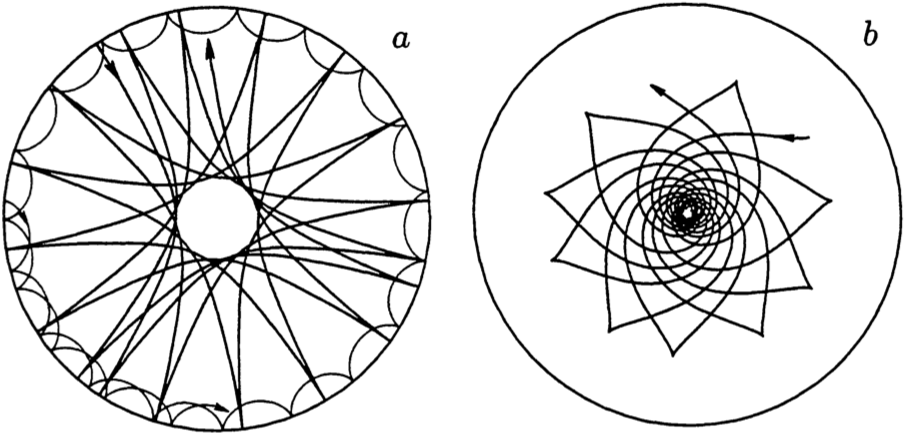
\includegraphics[keepaspectratio,width=0.7\textwidth]{raypath-gp}
\caption{(a): Percorso di due onda acustiche $p_8(l=2), p_8(l=100)$; (b): Percorso di un'onda di gravit\'a: $g_{10}(l=5)$. Da\cite{gou91seismic}.}\label{fig:raypathpg}
\end{figure}

Le frequenze dei modi sono determinate dalla condizione, per l fissato, che l'onda interferisca costruttivamente con se stessa; in figura (\ref{fig:raypathpg}) si mostra il percorso di di due onde acustiche (a) e un'onda di gravit\'a (b) racchiuse nelle cavit\'a di diversa profondit\'a. Un'onda stazionaria in direzione radiale implica che l'integrale di $k_r$ nella regione di propagazione fra due zeri consecutivi sia un intero multiplo di $\pi$:
\begin{equation}
\omega\int_{r_1}^{r_2}\sqrt{1-\frac{\omega_c^2}{\omega^2}-\frac{S_l^2}{\omega^2}(1-\frac{N^2}{\omega^2})}\,\frac{dr}{c}\approx\pi(n-\frac{1}{2})\label{eq:JWKBmode}
\end{equation}
che tiene conto del numero dei nodi radiali e dello sfasamento $\alpha$ prodotto nelle regioni di riflessione.

\begin{figure}[!ht]
\centering
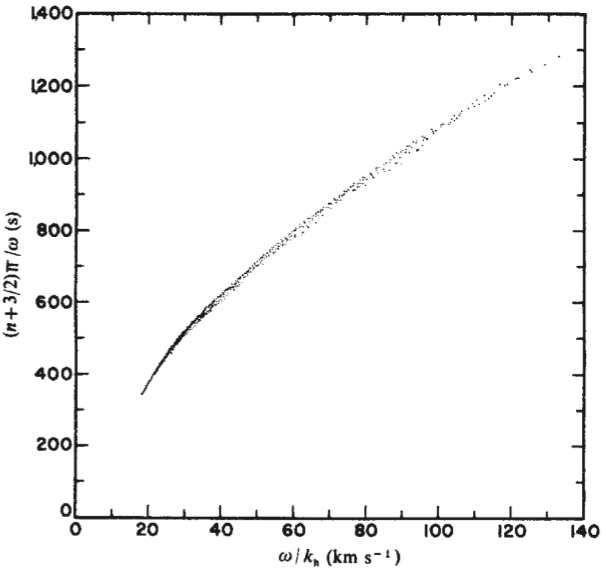
\includegraphics[keepaspectratio,width=0.5\textwidth]{dispersionDuvall}
\caption{I modi p sono allineati su un'unica curva, dove n \'e l'ordine radiale e $\alpha$ una fase dovuta alla riflessione. Da \cite{duv82dispersion}.}\label{fig:duv82dispersion}
\end{figure}

Questo comportamento \'e stato osservato per i modi p da \citet{duv82dispersion}. Un grafico di $\frac{\pi(n+\alpha(\omega))}{\omega}$ rispetto a $\frac{\omega}{k_h}$ rappresenta i modi p con un'unica curva (vedi \ref{fig:duv82dispersion}), per $\alpha$ opportuno con:
\begin{equation}
(n+\alpha(\omega))\frac{\pi}{\omega}=F(\frac{\omega}{k_h})=F(\frac{\omega}{L})\label{eq:duvallr}
\end{equation}
e usando la relazione di dispersione per onde acustiche \eqref{eq:approximatedispersion}
\begin{equation}
k_r^2=\frac{\omega^2}{c_s^2}(\frac{S_l^2}{\omega^2}-1)
\end{equation}
si ha:
\begin{align}
&F(w)=\int_{r_t}^R\sqrt{1-\frac{c_s^2}{r^2w^2}}\,\frac{dr}{c_s}\label{eq:duvallf}\\
&(n+\alpha)\pi\approx\int_{r_t}^Rk_r\,dr\approx\int_{r_t}^R\frac{\omega}{c_s}\sqrt{1-\frac{S_l^2}{\omega^2}}\,dr\label{eq:duvallexpli}
\end{align}

Utilizzando invece il limite per basse frequenze di \eqref{eq:approximatedispersion} per i modi g trovo la relazione di dispersione approssimata per $l\neq0$:
\begin{equation}
k_r^2=\frac{S_l^2}{c^2}(\frac{N^2}{\omega^2}-1)\label{eq:dispersionag}
\end{equation}
%[introdotta in precedenza \eqref{eq:bvf}]
e ottengo l'espressione analoga di \eqref{eq:duvallexpli} per i modi g:
\begin{equation}\label{eq:duvallg}
\frac{(n+\alpha_g)\pi}{L}\approx\int_{r_1}^{r_2}(\frac{N^2}{\omega^2}-1)\expy{\frac{1}{2}}\,d\ln{r}
\end{equation}
con $r_2\approx R_{cz}$ e $\alpha_g$ \'e una fase dovuta alla riflessione e dipende dall'andamento di $N^2$ nella regione di inversione del moto, alla base della zona convettiva.

\section{Espressioni asintotiche delle frequenze dei modi}

%Per alte frequenze trascuro N in \eqref{eq:JWKBmode}
%\begin{align*}
%&\omega\int_{r_1}^{r_2}\sqrt{1-\frac{\omega_c^2}{\omega^2}-\frac{S_l^2}{\omega^2}}\,\frac{dr}{c}\approx\pi(n-\frac{1}{2})\intxt{con $r_1=r_t$, $r_2=R_t$, e $\alpha(\omega)$ funzione della frequenza e del comportamento vicino alla superficie di $\omega_c$ e nella regione in cui $\omega\approx S_l$. Ritrovo la relazione di Duvall \eqref{eq:duvallr}.}
%\end{align*}

Per modi di alto grado angolare, confinati nella regione convettiva, considerando $\Gamma_1$ e $g$ lentamenta variabili e una stratificazione adiabatica, ottengo l'espressione delle frequenze dei modi approssimata:
\begin{equation}
\omega^2=\frac{2}{\mu_p}\frac{g}{\rsun{}}(n+\alpha)L
\end{equation}
dove $\mu_p=\frac{1}{\Gamma_1-1}$ \'e l'inidce politropico efficace della regione considerate.

I modi di basso l penetrano in profondit\'a, quindi approssimo $r_t\approx0$, e, espandendo \eqref{eq:duvallf} al primo'ordine in $\invers{w}$
\begin{equation}
F(w)\approx\int_0^R\frac{dr}{c}-w\expy{-1}\frac{\pi}{2}\label{eq:Flinear}
\end{equation}
 risulta
\begin{equation}
\int_0^R\frac{dr}{c}-\frac{L}{\omega}\frac{\pi}{2}=\frac{(n+\alpha)\pi}{\omega}
\end{equation}
e quindi le  frequenze sono equispaziate in n e $\nu_{nl}\approx\nu_{n-1,l+2}$ (per le deviazioni da questa uguaglianza, vedi \eqref{eq:tassoul}):
\begin{equation}
\nu_{nl}=\frac{\omega_{nl}}{2\pi}\approx(n+\frac{l}{2}+\frac{1}{4}+\alpha)\Delta\nu\label{eq:freqequi}
\end{equation}
con $\Delta\nu=[2\int_0^R\frac{dr}{c}]\expy{-1}\approx\SI{136}{\micro\hertz}$.

Questo comportamento a bassi l \'e stato osservato da \cite{cla79solar} sulla luce integrata sul intero disco solare.

%Le osservazioni della luce integrata sull'intero disco selezionano modi di basso grado angolare: \citet{cla79solar} osservano nello spettro Doppler (linee di assorbimento di K neutro: \SI{769.9}{\nano\meter}) della luce integrata sull'intero disco solare dei picchi equi-spaziati circa \SI{68}{\micro\hertz} interpretate come modi p di alto ordine n e basso grado l. I modi di basso ordine radiale l penetrano in profondit\'a e quindi portano informazioni sulle regioni di fusione e la loro evoluzione.

I modi g di alto n e basso l soddisfano un'equazione analoga a \eqref{eq:freqequi} con periodi equispaziati
\begin{equation}
\omega=\frac{L\int_{r_1}^{r_2}N\frac{dr}{r}}{\pi(n+\frac{l}{2}+\alpha_g)}
\end{equation}
e $\lim_{n\to\infty}{\alpha_g}\approx-\midfrac{1}{6}$.

%[Inserisci figura khomeagisot]
%[Inserisci figura pgmodesC]


{\let\clearpage\relax\let\cleardoublepage\relax
\chapter{Campo di velocit\'a solare.}
}

\section{Analisi fenomeni stazionari stocastici}

%\begin{wrapfigure}[25]{r}{0.4\textwidth}
%\centering
%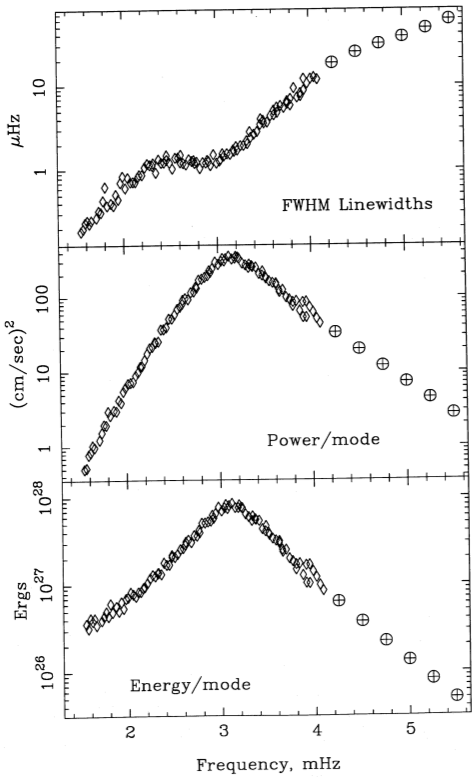
\includegraphics[keepaspectratio,width=0.4\textwidth]{modespheomenology}
%\caption{FWHM per i modi osservati, $V_{nl}$, energia totale per modi con $l\approx20$. Da \cite{libbrecht1988solar}.}\label{fig:modespheomenology}
%\end{wrapfigure}

\begin{wrapfigure}[16]{r}{0.5\textwidth}
\centering
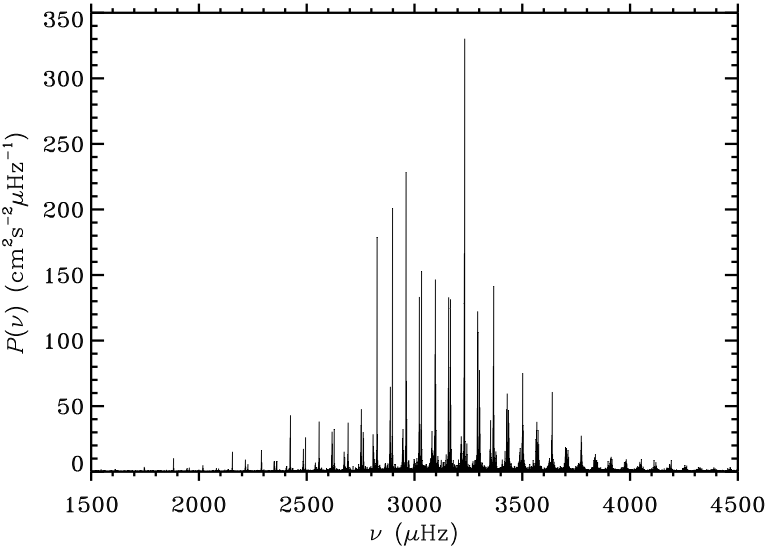
\includegraphics[keepaspectratio,width=0.48\textwidth]{lowlmodes}
\caption{Densit\'a spettrale modi p di basso grado angolare. Da \cite{chr02helioseismology}.}\label{fig:lowlmodes}
\end{wrapfigure}

I fenomeni periodici sulla superficie solare sono osservabili tramite tecniche fotometriche o spettroscopiche: una parte basilare dell'informazione contenuta nei modi di oscillazione \'e ricavata analizzando  lo spostamento Doppler delle righe di assorbimento dei metalli presenti negli strati visibili del sole.

L'ampiezza della velocit\'a di oscillazione per il singolo modo \'e  al pi\'u \SI{15}{\cm\per\second} quindi l'effetto doppler causa uno shift, al massimo, di $\frac{\Delta\lambda}{\lambda}\approx\num{e-10}$. Le misure Doppler su luce integrata sull'intero disco solare sono effettuate tramite uno spettroscopio a scattering risonante, in cui lo splitting  Zeeman dovuto a un campo magnetico esterno applicato a vapori di $Na/K$ permette la trasmissione  in due bande molto strette simmetriche rispetto alla linea spettrale di cui si vuole misurare lo shift: la velocit\'a Doppler \'e proporzionale alla differenza di intesit\'a osservata nelle due bande. Il tacometro di Fourier \'e uno degli strumenti pi\'u utilizzati per misure Doppler  con risoluzione spaziale.

\begin{workout}[Tachometro di Fourier]

\end{workout}

%Linee altezza formazione Diminuzione T formazione atomo? Diminuzione pressione minori collisioni?
% Na $D$ lines: $\lambda=\SI{589.6}{\nano\meter},\SI{589.0}{\nano\meter}$; SOHO (MDI): Ni \SI{678.8}{\nano\meter}; K Fraunhofer line \SI{770}{\nano\meter}; Ca \SI{643.9}{\nano\meter}; K \SI{769.9}{\nano\meter}

Il segnale Doppler osservato \'e proporzionale a:
\begin{equation}
    V_D(\theta,\phi,t)=\sin{\theta}\cos{\phi}\sum_{n,l,m}A_{nlm}c_{lm}P_l^m(\cos{\theta})\cos{(m\phi-\omega_{nlm}t-\beta_{nlm})}
\end{equation}
dove i coefficienti $c_{nl}$ descrivono la sensibilit\'a dello strumento ai singoli modi.

Il fattore $\sin{\theta}\cos{\phi}$ deriva dalla proiezione della velocit\'a radiale sulla linea di vista: i modi con periodo attorno ai 5 minuti di grado l non elevato causano uno spostamento quasi totalmente radiale:
\begin{align}
&\frac{\delta h|_{rms}}{\delta r|_{rms}}=\frac{\sqrt{l(l+1)}}{\sigma^2}\intxt{per oscillazioni con periodo intorno a \SI{5}{\minute} \'e}
&\sigma^2=\frac{\rsun{}^3}{G\msun{}}\omega^2\approx1000
\end{align}


\begin{workout}[rms displacement]

\begin{align}
&\delta r|_{rms}=\exv{\vec{\xi}\cdot\hat{r}}=\frac{1}{2}|\tilde{xi}_r|^2\\
&=\frac{1}{\Pi}\int_0^{\pi}\,dt\frac{1}{4\pi}\oint\Re{\tilde{\xi}_rY_{l,m}(\theta,\phi)\exp{-i\omega t}}^2\,d\omega\\
&\delta h_{rms}^2=\exv{|\vec{\xi}_h|^2}=\frac{1}{2}l(l+1)|\tilde{\xi}_h(r)|^2\\
&\frac{\delta h|_{rms}}{\delta r|_{rms}}=\frac{\sqrt{l(l+1)}}{\sigma}
\end{align}

\end{workout}

Per isolare il contributo di una singola $Y_{l_0m_0}$ considero
\begin{equation}\label{eq:dopplerTS}
V_{l_0m_0}(t)=\int_AV_D(\theta,\phi,t)W_{l_0m_0}(\theta,\phi)\,dA=\sum_{n,l,m}S_{l_0m_0,lm}A_{nlm}(t)\cos{(\omega_{nlm}t+\beta_{nlm,L_0m_0})}
\end{equation}
e ho integrato sul disco solare. $S_{l_0m_0,lm}$ \'e la funzione di risposta che non \'e esattamente $\propto\delta_{ll_0}\delta_{mm_0}$ poich\'e le armoniche sferiche sono ortogonali sull'intera sfera ma contiene contributi da valori di $(l,m)$ vicini e $W_{l_0m_0}\approx Y_{l_0m_0}$.

Considero la trasformata di Fourier di \eqref{eq:dopplerTS} per tempo di osservazione $T$
\begin{equation}
V_{l_0m_0}(\nu)=\int_{-\midfrac{T}{2}}^{\midfrac{T}{2}}V_{l_0m_0}(t)\exp{i2\pi\nu t}\,dt
\end{equation}

\begin{errata}[regioni in cui \'e concentrata la potenza]
La trasformata di Fourier della sequenza temporale di velocit\'a Doppler acquisita permette l'identificazioni nel diagramma $l-\nu$ le regioni in cui \'e concentrata la potenza.

La trasformata di Fourier di $V_{l_0m_0}(t)$ permette di isolare i modi come picchi nello spettro di potenza:
\begin{equation}
P(\omega,l,m)\propto|A_{nlm}|^2(\omega)
\end{equation}

\end{errata}

Un segnale di durata T permette una risoluzione $\Delta\omega=\frac{2\pi}{T}$ mentre il limite superiore delle frequenze osservate \'e dato dalla frequenza di Nyquist $\omega_{Ny}=\frac{\pi}{\Delta t}$ con $\Delta t$ risoluzione temporale; nel caso le dimensioni lineari $L_i$ della regione osservata siano piccole da poter trascurare la curvatura si hanno analoghe relazioni per le variabili spaziali cartesiane e vettore d'onda associato:
\begin{equation}
\Delta\omega=\frac{2\pi}{T}\leq\omega\leq\frac{\pi}{\Delta t},\ \Delta k_i=\frac{2\pi}{L_i}\leq k_i\leq\frac{\pi}{\Delta x_i}
\end{equation}

I modi normali sono identificati tramite la distribuzione spaziale delle oscillazioni in superficie, cio\'e tramite $(l,m)$ o, approssimando localmente l'oscillazione con un onda piana, tramite $k_h$, con
\begin{equation}
\vec{k}=k_r\hat{r}+\vec{k}_h,\ k_h^2=\frac{l(l+1)}{r^2}
\end{equation}
e dalla distribuzione delle frequenze, che identifica l'ordine n ovvero il numero di zeri radiali dello spostamento perturbato.

\begin{wrapfigure}[20]{r}{0.3\textwidth}
\centering
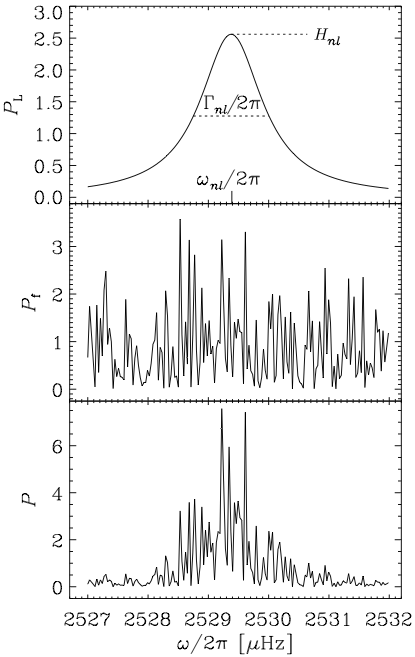
\includegraphics[keepaspectratio,width=0.3\textwidth]{Powerspectraldensity}
\caption{Densit\'a spettrale di oscillatore smorzato di frequenza naturale $\midfrac{\omega_{nl}}{2\pi}$ con forzante stocastica. $P_f$ \'e la DSP della forzante. $P=P_fP_L$. Da \cite{houdek2006stochastic}.}\label{fig:Powerspectraldensity}
\end{wrapfigure}

Considero un processo stocastico $x(t)$ campionato per un tempo T. Definisco la densit\'a spettrale di potenza (DSP) $P_T(\nu)$:
\begin{align}
&\frac{1}{T}|X_T(\nu)|^2\label{eq:powerspectraldensity}
%&S_T(\nu)=\frac{1}{T}\int_{-T/2}^{T/2}\int_{-T/2}^{T/2}x(t)x(t')\exp{i2\pi\nu t}\exp{i2\pi\nu t}\,dt\,dt'\\
=\int_{-T/2}^{T/2}\left[\frac{1}{T}\int_{-T/2}^{T/2}x(t')x(t'+\tau)\,dt'\right]\exp{i2\pi\nu \tau}\,d\tau\intxt{e, definendo la funzione di autocorrelazione $C_T(\tau)$, si ha}
&P_T(\nu)=\int_{-T/2}^{T/2}C_T(\tau)\exp{i2\pi\nu\tau}\,d\tau\\
&C(\tau)=E(x(t)x(t+\tau))=\lim_{T\to\infty}{C_T(\tau)}
\end{align}

\begin{wrapfigure}[24]{r}{0.3\textwidth}
\centering
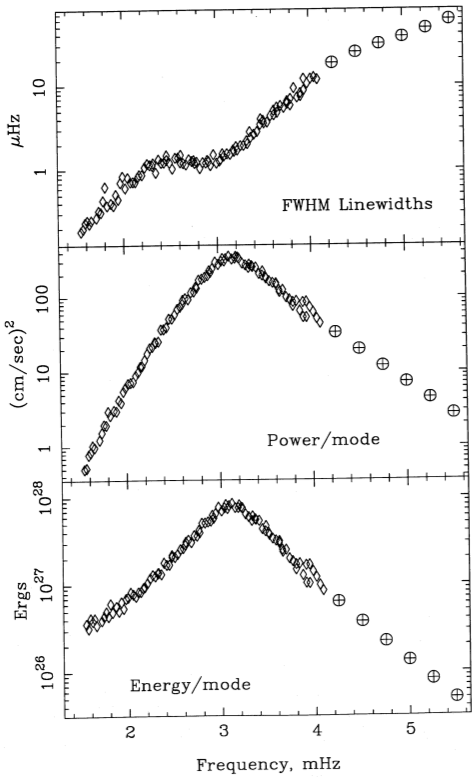
\includegraphics[keepaspectratio,width=0.3\textwidth]{modespheomenology}
\caption{Risultati osservativi per $\Gamma$, $\exv{V^2}$ e $E_{nl}$ in funzione della frequenza per modi con $l\approx20$. Da \cite{libbrecht1988solar}.}\label{fig:Powerspectraldensity}
\end{wrapfigure}

Il valore di aspettazione della densit\'a spettrale per un tempo di osservazione tendente a infinito \'e
\begin{align}
&P_x(\nu)=\lim_{T\to\infty}{E[P_T(\nu)]}=\int_{-\infty}^{-\infty}C(\tau)\exp{2\pi i\nu\tau}\,d\tau\intxt{da cui si ha il teorema di Wiener-Khinchin}
&C(\tau)=\int_{-\infty}^{-\infty}P_x(\nu)\exp{-2\pi i\nu\tau}\,d\nu\intxt{che per $\tau=0$ da l'identit\'a di Parseval}
&C(0)=\int_{-\infty}^{-\infty}P_x(\nu)\,d\nu=E(x^2)
\end{align}

\begin{workout}[Asteroseismology: data analysis - Il segnale solare osservato \'e sovrapposizione di un segnale armonico e del rumore]
Il segnale solare osservato \'e sovrapposizione di un segnale armonico e del rumore: la densit\'a spettrale si scrive
\begin{equation}
P_x(\nu)=P_{osc}(\nu)+P_n(\nu)=\sum_{n,l,m}H_nV_l^2c_{l,m}L(\frac{\nu-\nu_{nlm}}{\Gamma_{nlm}})+\sum_i\frac{H_i}{1+(2\pi\tau_i\nu)^{b_i}}
\end{equation}
dove $H_n$ \'e l'altezza del picco $\Gamma_{nlm}$ la larghezza a met\'a altezza del picco. La seconda sommatoria descrive il rumore solare e strumentale.
\end{workout}

Il segnale solare osservato \'e sovrapposizione di un segnale armonico e del rumore. La densit\'a spettrale si scrive, usando l'indice ${\alpha}$ per indintificare i modi normali
\begin{equation}
P_x(\nu)=\sum_i\frac{H_{\alpha}B_i\midfrac{\Gamma^2_{\alpha}}{4}}{(\nu-\nu_{\alpha}-\Delta\nu_i)^2+\midfrac{\Gamma^2_{\alpha}}{4}}+P_n(\nu)
\end{equation}
dove $H_{\alpha}$ \'e l'altezza del picco, $\Gamma_{\alpha}$ la larghezza a met\'a altezza, i termini $\Delta\nu_i$ e $B_i$ descrivono i picchi parassiti dovuti a interruzioni della serie temporale; il secondo termine descrive il rumore solare e strumentale.

Il profilo lorentziano della densit\'a spettrale del segnale periodico \'e giustificata assumendo che le ampiezze superficiali dei modi obbediscano all'equazione del moto di un oscillatore armonico smorzato con forzante stocastica. Determino la densit\'a spettrale dell'oscillatore
\begin{equation}
M_{\alpha}[\TtwoDy{t}{\vec{\xi}_{\alpha}}+\Gamma_{\alpha}\TDy{t}{\vec{\xi}_{\alpha}}+\omega_{\alpha}^2\vec{\xi}_{\alpha}]=\vec{F}(t)
\end{equation}
con $\midfrac{\Gamma_{\alpha}}{2}$ costante di smorzamento, inverso del tempo di vita, $\omega_{\alpha}$ frequenza del modo adiabatico e $\vec{F}$ forzante stocastica.
%=\Im{\omega}$

\begin{workout}[P quadro ampiezza FT vs PSD]

\end{workout}

Assumendo $\omega_{\alpha}\gg\Gamma_{\alpha}$, cio\'e gli scambi di energia tra i modi normali e i moti turbolenti in superficie hanno tempo caratteristico $\tau_{nad}\gg\Pi_{osc}$, lo spettro in frequenza dell'oscillatore $P(\omega)=\exv{|\xi_{\alpha}(\omega)|^2}$,vicino a $\omega_{\alpha}$ \'e della forma:
\begin{equation}
P(\omega)\propto P_LP_f=\frac{\midfrac{\Gamma_{\alpha}}{2\pi}}{(\omega-\omega_{\alpha})^2+\midfrac{\Gamma_{\alpha}}{4}}P_f
\end{equation}

L'energia dell'oscillatore varia su tempi scala proporzionali a $\invers{\Gamma}_{\alpha}$ attorno al valor medio $\bar{E}_{\alpha}$:
\begin{align}
&\TDy{t}{E_{\alpha}}+\Gamma_{\alpha}E_{\alpha}=\exv{\dvec{\xi}_{\alpha}\cdot\vec{F}}\\
&\bar{E}_{\alpha}=\frac{\exv{\dvec{\xi}_{\alpha}\cdot\vec{F}}}{\Gamma_{\alpha}}
\end{align}
dove $\exv{\dvec{\xi}_{\alpha}\cdot\vec{F}}$ \'e il lavoro della forzante mediato su un periodo.

Il valore di aspettazione dell'energia totale di un modo si ottiene dalle osservazioni tramite:
\begin{equation}
\bar{E}_{\alpha}=M_{\alpha}V_{\alpha}^2=M_{\alpha}\frac{1}{T_{obs}}\int_{-\infty}^{\infty}|V(\nu)|^2\,d\nu\propto M_{\alpha}\Gamma_{\alpha}A_{\alpha}
\end{equation}
dove $H_{\alpha}$ \'e l'altezza di picco della densit\'a spettrale di potenza per $V_{\alpha}(\nu)$. In figura (\ref{fig:Powerspectraldensity}) si mostrano $V_{\alpha}^2$ e $\Gamma_{\alpha}$ osservati e l'energia totale del modo in funzione della frequenza.

\begin{workout}[Energia totale del modo (in fenomeni stazionari stocastici)]
L'energia totale di un modo \'e
\begin{align}
&E_{(n,l)}=\int_0^M\,dm\exv{\dvec{\xi}^2_{nl}}
%E_{\omega_0}=\int_0^M\exv{v_{osc}^2}
\intxt{e avendo normalizzato i modi in maniera opportuna si ha}
&E_{nl}=I_{nl}V_{nl}^2=\frac{1}{2}I_{nl}\omega_{nl}^2A_{nl}^2
\end{align}
dove $V_{nl}^2$ e $A_{nl}^2$ sono il valore quadratico medio della velocit\'a e dell'ampiezza dell'oscillazione in superficie. In figura (\ref{fig:Powerspectraldensity}) si mostrano $V_{\alpha}^2$ e $\Gamma_{\alpha}$ osservati e l'energia totale del modo.

\end{workout}

\begin{workout}[Velocity rms energy width: Solar p-modes phenomenolog]
\begin{wrapfigure}[25]{r}{0.4\textwidth}
\centering
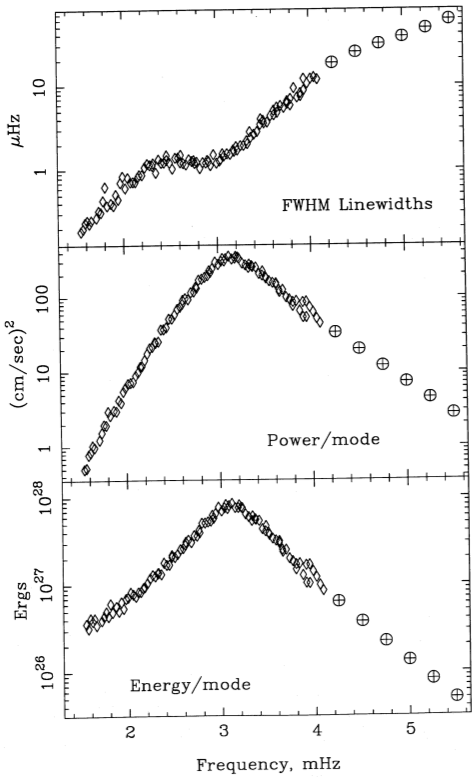
\includegraphics[keepaspectratio,width=0.4\textwidth]{modespheomenology}
\caption{$\exv{P}=|A(\omega)|^2$ spettro di oscillatore armonico forzato, smorzato di frequenza naturale $\midfrac{\omega_{nl}}{2\pi}$. Da \cite{libbrecht1988solar}.}\label{fig:Powerspectraldensity}
\end{wrapfigure}
\end{workout}

\begin{workout}[Power spectra doppler velocity]
\begin{equation}
P(\nu)=\frac{AB_i\midfrac{\Gamma^2}{4}}{(\nu-\nu_0-\Delta\nu_i)^2+\midfrac{\Gamma^2}{4}}
\end{equation}
\end{workout}

\begin{workout}[power $E\Gamma$-Howe hill komm 2000; Goldreich murray kumar 1994
]
Howe hill komm 2000; Goldreich murray kumar 1994
\end{workout}

\begin{errata}[Peak of $V(\nu)$ vs peak $A(\nu)$]

I parametri che descrivono il picco della densit\'a spettrale in corrispondenza all'autofrequenza $\nu_{nlm}$ sono l'altezza di picco $H_{nl}$ e la larghezza a met\'a altezza, inverso del tempo di vita del modo
\begin{equation}
H_{nl}=\int_{\nu_0-\midfrac{\delta}{2}}^{\nu_0-\midfrac{\delta}{2}}|\tilde{V}(\nu)|^2\,d\nu,\ \delta=\midfrac{1}{T}
\end{equation}
e larghezza a met\'a altezza $\midfrac{\Gamma_{nl}}{2\pi}=\Delta_{nl}$ illustrato in \subref{fig:FWHMbison}.
\end{errata}




%\section{Descrizione dello spettro dei modi tramite oscillatori armonici}

\begin{errata}[modello per determinare l'ampiezza dei modi p ]

Un modello per determinare l'ampiezza dei modi p considera un insieme di oscillatori armonici di frequenze naturali $\omega_{nl}$, i modi normali, introduce uno smorzamento che tiene conto dell'interazione con moti turbolenti ed altri effetti e una forzante stocastica che tiene conto della generazione di onde, con spettro determinato da velocit\'a e dimensioni della corrente turbolenta, da parte dei moti convettivi superficiali; trascuro gli effetti non lineari e eventuali instabilit\'a intrinseche alle pulsazioni. La sorgente delle eccitazioni stocastiche \'e supposta vicino alla superficie solare ed i modi normali risultano da quelle onde per cui si ha interferenza costruttiva.

\end{errata}



%La funzione $f(t)$ contiene il contributo dei moti turbolenti e fluttuazioni entropia causati dai moti convettivi.

\begin{workout}[densit\'a spettrale dell'oscillatore]

Determino la densit\'a spettrale dell'oscillatore
\begin{equation}
I_{nl}[\TtwoDy{t}{\xi_{nl}}+\Gamma_{nl}\TDy{t}{\xi_{nl}}+\omega_0^2\xi_{nl}]=f(t)
\end{equation}

con $\midfrac{\Gamma}{2}=\Im{\omega}$ costante di smorzamento.

Assumendo $\omega_{nl}\gg\Gamma_{nl}$, cio\'e gli scambi di energia tra i modi e la turbolenza hanno tempo caratteristico $\tau_{nad}\gg\Pi_{osc}$, lo spettro in frequenza dell'oscillatore $P(\omega)=E[|\xi_{nl}(\omega)|^2]$ \'e della forma:
\begin{equation}
P(\omega)\propto P_LP_f=\frac{\midfrac{\Gamma_{nl}}{2\pi}}{(\omega-\omega_0)^2+\midfrac{\Gamma_{nl}}{4}}P_f
\end{equation}

%Poich\'e su tempi caratteristici delle osservazioni le caratterische dei modi sono costanti si pu\'o
%Modelling solar oscillation power spectra (ADH90): formula 2 ??
%\begin{equation}
%E_{nl}=\frac{1}{2}\exv{|\vec{\xi}_{nl}|^2}I_{nl}\omega_{nl}^2
%\end{equation}

L'energia dell'oscillatore varia su tempi scala proporzionali a $\invers{\Gamma}_{nl}$ attorno al valor medio $\bar{E}_{nl}$:
\begin{align}
&\TDy{t}{E_{nl}}+\Gamma_{nl}E_{nl}=\exv{\dvec{\xi}_{nl}\cdot\vec{F}}\\
&\bar{E}_{nl}=\frac{\exv{\dvec{\xi}_{nl}\cdot\vec{F}}}{\Gamma_{nl}}
\end{align}
dove $\exv{\dvec{\xi}_{nl}\cdot\vec{F}}$ \'e il lavoro della forzante mediato su un periodo.

\end{workout}


\begin{workout}[Energia totale del modo (in descrizione spettro dei modi tramite oscillatori armonici)]
\begin{align}
&E_{(n,l)}=\int_0^M\,dm\exv{\dvec{\xi}^2_{nl}}
%E_{\omega_0}=\int_0^M\exv{v_{osc}^2}
\intxt{e avendo normalizzato i modi in maniera opportuna si ha}
&E_{nl}=I_{nl}E[V_{nl}^2]=\frac{1}{2}I_{nl}\omega_{nl}E[A_{nl}^2]\\
&\propto I_{nl}\omega_{nl}\intsinf{}P(\omega)\,d\omega
\end{align}

\end{workout}
%
%E=Mv^2(\nu_0),\ M(r_s)=\frac{I}{\xi_r^2(r_s)}\intxt{$r_s$ raggio linea osservazione}
%&\propto\frac{P_f(\omega_{nl})}{\Gamma_{nl}}
%\begin{align}
%&H\approx\frac{2V_{rms}^2}{\eta}:\ T_{obs}\gg 2\tau\\
%&H\approx V_{rms}^2T_{obs}:\ T_{obs}\ll 2\tau
%\end{align}

\begin{errata}[power density height H, $P_f$]

Abbiamo le seguenti relazioni tra i parametri dei picchi spettrali:
\begin{align}
&V_{nl}^2=\frac{P_f}{\Gamma_{nl}I}=\frac{1}{4}\Gamma H_{nl}\\
&H_{nl}=\frac{P_f}{(\midfrac{\Gamma_{nl}}{2})^2I}
\end{align}

In \subref{fig:peakDmeasured} si mostra il buon accordo tra $H$ calcolato sulla base di questo modello, con $P_f$ determinato sulla base di un modello della convezione nelle regioni vicino alla superficie solare e $\Gamma$ ricavato dalle osservazioni, con l'altezza di picco misurata.

\begin{figure}[!ht]

\begin{subfigure}{0.49\textwidth}
\centering
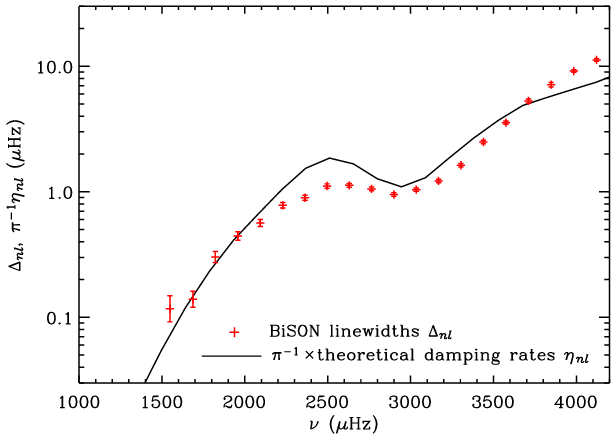
\includegraphics[keepaspectratio,width=0.9\textwidth]{FWHM}
\caption{FWHM per i modi di basso l. Da \cite{houdek2006stochastic}.}\label{fig:FWHMbison}
\end{subfigure}
~
\begin{subfigure}{0.49\textwidth}
\centering
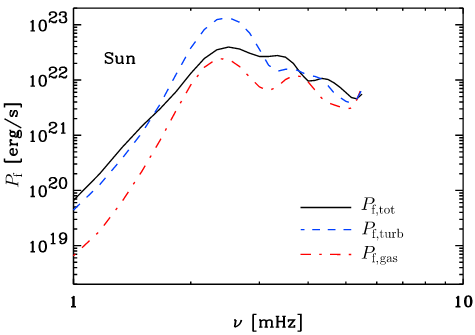
\includegraphics[keepaspectratio,width=0.9\textwidth]{Pf}
\caption{Eccitazione $P_f$ totale e contributi dovuti ai moti turbolenti e alle fluttuazioni nella pressione del gas. Da \cite{houdek2006stochastic}.}\label{fig:Pf}
\end{subfigure}
\centering
\begin{subfigure}[c]{0.7\textwidth}
\centering
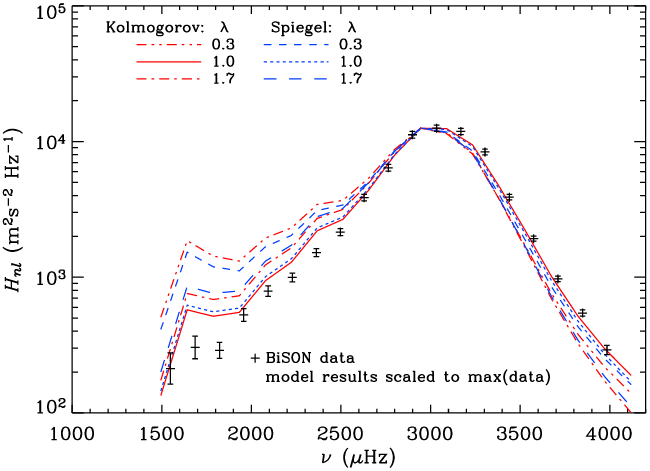
\includegraphics[keepaspectratio,width=0.99\textwidth]{HnlDmeasured}
\caption{Ampiezza dei modi $H_{nl}$. Le previsioni teoriche includono la larghezza del picco misurata sperimentalmente. Da \cite{houdek2006stochastic}.}\label{fig:peakDmeasured}
\end{subfigure}

\end{figure}

\end{errata}

%[Si ipotizza che le oscillazioni siano eccitate in maniera stocastica dai moti convettivi: la larghezza delle frequenze risonanti \'e determinata dal tempo di smorzamento.]
%[Extensive turbolent layers: stars lose all hint of vibrational instability]
%[Not self excited: driven to observable amplitude by external process]
%[Turbolent convection: source of pulsational energy, emit acustic radiation]
%[Stable pulsation: spectrum as that of an ensemble of harmonic oscillator stocastically driven and damped]
%[Power spectrum indipendent of l for $l<100$: low degree modes are not influenced by $k_h$. Vertical propagation: superficial layers (low l modes are generated in these strata)]
%[Interaction with turbolent convection]
%[Radiative transfer (as frequencies rise modes became more sensitive to rapid relaxation time in solar atmosphere)]
%[La stabilit\'a dei modi g \'e determinata dalla stabilit\'a convettiva: se non sono presenti regioni di instabilit\'a convettiva i modi g sono stabili ($g_+$), se esistono zone convettivamente instabili esistono anche modi g instabili ($g_{\,-}$).]
%[Excitation p-modes: fluctuating turbolent pressure (Raynold stresses). Excitation g-modes: nuclear burning instabilities. Damping: radiative losses, viscosity, nonlinear interaction between modes.]
%[Low l p-modes exponential decay with e-folding time several days.]

\section{Rotazione}

In presenza di un campo di velocit\'a $\vec{v}_0$ il termine d'inerzia $\rho_0\TDy{t}{\vec{v}}$ dell'equazione del moto per un elemento di fluido nel riferimento solidale \'e:
\begin{equation}
\rho_0(\PDof{t}+\scap{v_0}{\nabla})^2\vec{\xi}\label{eq:inertialtermvf}
\end{equation}

Il Sole \'e un rotatore lento: le osservazioni della superficie mostrano una dipendenza dalla co-latitudine (\cite{ulrich1988solar}) 
\begin{equation}
\frac{\Omega(\theta)}{2\pi}=\SI{451.5}{\nano\hertz}-\SI{65.3}{\nano\hertz}\cos^2{\theta}-\SI{66.7}{\nano\hertz}\cos^4{\theta}
\end{equation}

Il campo di velocit\'a rotazionale \'e 
\begin{equation}
\vec{v_0}=\vecp{\Omega}{r}
\end{equation}

Considero il termine dovuto alla rotazione come una piccola correzione alle frequenze dei modi
\begin{equation}
\omega_{n,l,m}=\omega_{(n,l)}+\Delta\omega_{(l,m)}
\end{equation}
Nel caso di rotazione uniforme \'e facile trovare le correzioni dovute alla rotazione: passando al SR corotante \[(r',\theta',\phi')=(r,\theta,\phi-\Omega t)\] e data la dipendenza delle oscillazioni dall'angolo azimutale e dal tempo deve essere \[\cos{(m\phi'-\omega_{n,l}t)}=\cos{(m\phi-\omega_{n,l,m}t)}\] cio\'e \[\Delta\omega_{(l,m)}=m\Omega\].

I modi di oscillazioni sono onde stazionarie nel rifermento corotante mentre nel riferimento inerziale si ha uno spostamento delle frequenze per le onde che hanno una componente parallela all'equatore; le onde prograde/retrograde ($m=\pm l$) hanno shift massimo. 

%Questo \'e spiegabile :
%Corotating frame: agreement between equation of motions vedi dalsnotes 8;
%\begin{align}
%&\cos{(m\phi'+m\Omega t-\omega t)}=\cos{(m\phi'-\omega't)}\\
%&(r',\theta',\phi')=(r,\theta,\phi-\Omega t)
%\end{align}
%con $\omega'=\omega-\Omega m$.
\begin{workout}[Doppler effect on frequency from advection]

\end{workout}

\begin{center}

\begin{minipage}{0.4\textwidth}
\captionof{figure}{Diagramma $\omega-k_h$ per osservazione di una regione solare $\ang{;;2}\times\ang{;;2}$ mediata in direzione nord-sud: la misura \'e maggiormente sensibile alle onde che si propagano in direzione est-ovest lungo l'equatore. Si osserva lo spostamento dovuto alla rotazione dalla predizione per modello non-rotante (linee continue). Da \cite{rhodes1979new}.}\label{fig:rotationshiftridge}
\end{minipage}
~
\begin{minipage}{0.35\textwidth}
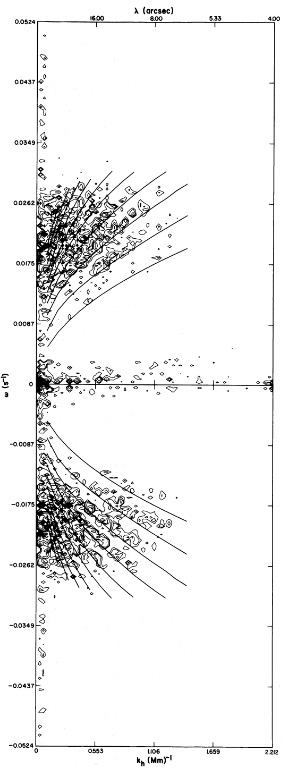
\includegraphics[keepaspectratio,angle=0,width=0.95\textwidth]{rotationshiftridge}
\end{minipage}

\end{center}

\'E possibile identificare l'effetto della rotazione effettuando una misura sensibile a onde con direzione di propagazione parallela all'equatore
\begin{equation}
\frac{\Delta\omega}{\omega}=\pm\frac{V_{adv}}{V_{ph}}
%&V_{adv}=\pm\frac{\Delta\omega}{k_h}
\end{equation}
che da una indicazione della velocit\'a media dovuta alla rotazione $V_{adv}$ nella regione in cui \'e confinato il modo con $V_{ph}=\frac{\omega}{k_h}$.

\begin{workout}[rotazione perturbazione frequenze modi]
Considero il termine dovuto alla rotazione $\vec{v_0}=\vecp{\Omega}{r}$ come una piccola correzione al modello che modifica le frequenze dei modi $\omega_{(l,m)}+\Delta\omega_{(l,m)}$.
\end{workout}

Lo splitting delle frequenze dei modi \'e determinato considerando l'equazione del moto al primo ordine nella perturbazione, con $\alpha=(l,m)$:
\begin{equation}\label{eq:eomrotation}
\rho_0(\omega_{\alpha}^2+2\omega_{\alpha}\delta\omega_{\alpha})\vec{\xi}=\nabla P_1-\frac{\rho_1}{\rho_0}\nabla P_0+\rho_0\nabla\Phi_1+2i\omega_{\alpha}\rho_0(\scap{v_0}{\nabla})\vec{\xi}
\end{equation}
dove ho esplicitato il termine inerziale \eqref{eq:inertialtermvf} e usando $(\scap{v_0}{\nabla})\vec{\xi}=im\Omega\vec{\xi}+\vecp{\Omega}{\xi}$, lo splitting dovuto alla rotazione \'e:
\begin{equation}\label{eq:splitfreqrotation}
\delta\omega_{\alpha}=\frac{i\int\rho_0\xi_{\alpha}^*(\scap{v_0}{\nabla})\xi_{\alpha}\,d^3x}{\int\rho_0\xi_{\alpha}^*\xi_{\alpha}\,d^3x}=\frac{-m\int\rho_0\vec{\Omega}(r,\theta)\cdot\vec{\xi}_{\alpha}^*\xi_{\alpha}\,d^3x+i\int\rho_0\vec{\xi}_{\alpha}^*(\vecp{\Omega}{\xi_{\alpha}})\,d^3x}{\int\rho_0\xi_{\alpha}^*\xi_{\alpha}\,d^3x}
\end{equation}

%Per rotazione puramente radiale $\Omega(r)$ la relazione tra lo splitting delle frequenze e la rotazione \'e
%\begin{equation}
%\Delta\omega_{\alpha}=-m\frac{\int_0^{\rsun{}}\rho_0\Omega\{|\xi_r-\xi_h|^2+[l(l+1)-2]|\xi_h|^2\}r^2\,dr}{\int_0^{\rsun{}}\rho_0\{|\xi_r|^2+l(l+1)|\xi_h|^2\}r^2\,dr}=\int_0^{\rsun{}}K_{\alpha}(r)\Omega(r)\,dr
%\end{equation}
%Any given $\Delta\omega_{\alpha}$ samples angular velocity in the depth range corresponding to $\xi_{\alpha}$.

La velocit\'a angolare contribuisce a $\Delta\omega_{\alpha}$ negli strati in cui $\xi_{\alpha}$ \'e apprezzabile. Nel caso di rotazione dipendente solo da r si ha che $\Delta\omega_{\alpha}$ \'e lineare in m: ho $2l+1$ frequenze equispaziate e per modi p di alto n approssimo lo splitting delle frequenze con:
\begin{align}
&\delta\omega_{nlm}\approx m\frac{\int_{r_t}^R\Omega(r)\,\frac{dr}{c_s}}{\int_{r_t}^R\frac{dr}{c_s}}\intxt{per $\Omega(r)$ puramente radiale, cio\'e  per una media sulla latitudine; per velocit\'a angolare generale $\Omega(r,\theta)$, usando le propriet\'a dei polinomi di Legendre $P_l^m(x)$:}
&\delta\omega_{nlm}\approx m\frac{\int_{\cos{\Theta}}^{-\cos{\Theta}}(\cos^2{\Theta}-\cos^2{\theta})\expy{-\frac{1}{2}}\int_{r_t}^R(1-\frac{L^2c^2}{r^2\omega^2})\expy{\frac{1}{2}}\Omega(r,\theta)\frac{dr}{c}\,d(\cos{\theta})}{\int_{r_t}^R(1-\frac{L^2c_s^2}{r^2\omega^2})\expy{\frac{1}{2}}\,\frac{dr}{c_s}}\intxt{dove}
&\Theta=\sin^{-1}{(\frac{m}{L}).}
\end{align}

Le autofunzioni hanno ampiezza apprezzabile nella fascia compresa tra le latitudini $\pm\Theta$: questo permette la risoluzione  della dipendenza da $\theta$ della rotazione.
Per determinare quindi la rotazione si utilizzano tecniche di inverzione basate sul principio variazionale
%Per rotazione puramente radiale $\Omega(r)$ la relazione tra lo splitting delle frequenze e la rotazione \'e
%\begin{equation}
%\Delta\omega_{\alpha}=-m\frac{\int_0^{\rsun{}}\rho_0\Omega\{|\xi_r-\xi_h|^2+[l(l+1)-2]|\xi_h|^2\}r^2\,dr}{\int_0^{\rsun{}}\rho_0\{|\xi_r|^2+l(l+1)|\xi_h|^2\}r^2\,dr}=\int_0^{\rsun{}}K_{\alpha}(r)\Omega(r)\,dr
%\end{equation}
%Any given $\Delta\omega_{\alpha}$ samples angular velocity in the depth range corresponding to $\xi_{\alpha}$.
e poich\'e non \'e sempre possibile misurare lo splitting in m si parametrizzano le frequenze nel multipletto $(n,l)$ tramite:
\begin{equation}
\nu_{nlm}=\nu_{nl0}+\sum_{j=1}^{j_{\max}}a_j(n,l)\pol_j^{(l)}(m)\label{eq:freqmulti}
\end{equation}
e ricavo i coefficienti tramite fit con le frequenze osservate; i coefficienti dispari contengono il contributo della rotazione al termine lineare, i coefficienti pari effetti delle asfericit\'a nella struttura solare e effetti quadratici della rotazione.

\end{document}